\documentclass[12pt,twoside=off,
bibliography=totoc,listof=totoc,appendixprefix,paper=a4,headings=small]{scrbook}

\usepackage[
  paper=a4paper,
  left=40mm,
  right=25mm,
  top=20mm,
  bottom=20mm,
  bindingoffset=0mm]{geometry}
\setlength{\footskip}{15mm}
\usepackage{mathptmx}
\usepackage{float}
\usepackage{graphicx,adjustbox} 
\KOMAoptions{parskip=half}

\renewcommand{\footnotesize}{\fontsize{10}{12}\selectfont}

\RedeclareSectionCommand[
  beforeskip=1.5\baselineskip,
  afterskip=0.5\baselineskip,
  font=\fontsize{14}{16}\bfseries
]{section}

\RedeclareSectionCommand[
  beforeskip=0.5\baselineskip,  
  afterskip=0.5\baselineskip
]{chapter}

\usepackage{cite}            
\usepackage{amsfonts} 
\usepackage[utf8]{inputenc}         
\usepackage{ngerman}				
\usepackage[T1]{fontenc}
\usepackage{lmodern}				
		
\setkomafont{disposition}{\bfseries}
\RedeclareSectionCommand[
  beforeskip=1.5\baselineskip,
  afterskip=0.5\baselineskip,
  font=\fontsize{14}{16}\bfseries
]{section}


\usepackage{graphicx} 				
\graphicspath{{./Bilder/}}          

\usepackage{url}					
\usepackage[colorlinks,linkcolor=black,citecolor=black,urlcolor=black]{hyperref} 	
\usepackage{tabularx} 				
\usepackage{longtable}
\usepackage{multicol}
\usepackage{multirow}
\usepackage{booktabs}
\usepackage{tabularx}

\usepackage[active]{srcltx}

\usepackage{listings}		

\usepackage{mdwlist}				

\usepackage{setspace} 			
\newtheorem{mydef}{Merksatz}  	
\newtheorem{bsp}{Beispiel}
		
\usepackage{lscape}		
\usepackage{amsmath}	
\usepackage{calc}

\usepackage{footnote}		
\renewcommand{\footnotesize}{\fontsize{10}{12}\selectfont}

\usepackage{tablefootnote}			
\usepackage{microtype}		
\setlength{\abovecaptionskip}{3pt}
\setlength{\belowcaptionskip}{3pt}
\makeatletter
  % Abstand oberhalb eines Floats auf Float-Seiten (nur [t] oder reine Float-Seiten)
  \setlength{\@fptop}{0pt}      
  % Abstand unterhalb eines Floats auf Float-Seiten
  \setlength{\@fpbot}{0pt}      
  % Abstand zwischen zwei Floats auf Float-Seiten
  \setlength{\@fpsep}{5pt}      
\makeatother

% optional: Abstand Text ↔ Float [t] oder [b] noch weiter reduzieren
\setlength{\textfloatsep}{6pt plus 1pt minus 1pt}
\hyphenation{voll-st\"andigen}		
\setcounter{tocdepth}{1}		
\begin{document}

\frontmatter
    % Titelseite ohne Kopf- oder Fußzeile
\thispagestyle{empty}

% Alle Elemente zentriert
\begin{center}

% Vertikale Anpassung für bessere Platzierung
\vspace*{0.5cm}

% Hochschullogo

\includegraphics[width=0.6\linewidth]{Bilder/hochschule-ansbach@2x-3326483176.png}

\vspace{1.5cm}

% Art der Arbeit
{\LARGE \textbf{Bachelorarbeit}}\\ 

\vspace{1.5cm}

% Titel der Arbeit 
{\Large \textbf{Simulation einer Predator und Prey Umgebung \\ und Trainingsszenarien für optimiertes Verhalten \\ durch Reinforcement Learning}}\\ 

\vspace{2cm}

% Name des Autors
{\Large \textbf{Fynn Madrian}}\\[1.5cm]

% Metadaten
{\large
\begin{tabular}{r l}
  Gutachter:    & Geißelsöder, Prof. Dr. Stefan \\
  & \\
  Semester:     & Sommersemester 2025 \\
  & \\
  Verfasser:    & Fynn Madrian \\
  & \\
  Matrikel-Nr.: & 00163467 \\
  & \\
  E-Mail:       & f.madrian18230@hs-ansbach.de \\
  & \\
  Studienfach:  & Künstliche Intelligenz und Kognitive Systeme \\
  & \\[0.5cm]
  \textbf{Abgabetermin:} & \textbf{15. Juli 2025} \\
\end{tabular}
}

% Vertikaler Ausgleich nach unten
\vspace*{\fill}

\end{center}
 			% Titelblatt
    \thispagestyle{plain}
\begin{center}
  \textbf{\Large Erklärung}
\end{center}

\begin{quote}
„Ich versichere, dass ich die Arbeit selbstständig angefertigt, nicht anderweitig für 
Prüfungszwecke vorgelegt, alle benutzten Quellen und Hilfsmittel angegeben sowie 
wörtliche und sinngemäße Zitate gekennzeichnet habe.“
\end{quote}

\vfill

\noindent
\begin{minipage}[t]{0.45\textwidth}
\textbf{Ort, Datum:} \hrulefill
\end{minipage}%
\hfill
\begin{minipage}[t]{0.45\textwidth}
\textbf{Unterschrift:} \hrulefill
\end{minipage}
 	% Abstract auf Deutsch
    \newpage
    \vspace*{1cm}
\addcontentsline{toc}{chapter}{Abstract}
\begin{center}
    \textbf{Abstract}
\end{center}

\vspace*{1cm}
Diese Arbeit untersucht modulare Trainingsstrategien zur Verbesserung des Verhaltens von Reinforcement-Learning-Agenten in komplexen Überlebensszenarien. Ausgehend von instabilen Multi-Agent-Experimenten wird das Gesamtproblem für Single-Agenten in einzelne Aufgaben wie Navigation, Exploration und Flucht aufgeteilt. Diese Subtasks werden separat trainiert, feinjustiert und anschließend in ein vollumfängliches Survival-Szenario übertragen. Die Analyse zeigt, dass sowohl das Szenariodesign als auch die Wahl der Rewardfunktionen zentral für stabiles Lernen sind. Curriculum Learning durch schrittweise gesteigerte Komplexität fördert dabei robuste Strategien und ermöglicht eine effektivere Nutzung zuvor erlernter Fähigkeiten.

Während vortrainierte Modelle vergleichbare Gesamtperformance zum Training-from-Scratch erreichen, behalten sie jeweils charakteristische Strategiemuster aus ihrem Subtask-Kontext bei – ein Effekt, der gezielt zur Steuerung spezifischer Verhaltensweisen genutzt werden kann. Eine anschließende Retention-Analyse bestätigt, dass einige Spezialfähigkeiten durch das Fine Tuning erhalten bleiben, während andere – insbesondere bei widersprüchlichen Zielen – verdrängt werden. Zusätzlich wird gezeigt, dass die Generalisierungsfähigkeit der Agenten stark von der Komplexität der Subtask-Umgebung abhängt: Modelle, die in strukturell anspruchsvollen Szenarien trainiert wurden, entwickelten robustere Taktiken und konnten diese besser auf neue Umgebungen übertragen.

Die Evaluation erfolgt dabei nicht nur über aggregierte Rewards, sondern anhand spezifischer Metriken wie Zeit zum Ziel, Überlebensdauer und Erfolgsrate. Die Ergebnisse legen nahe, dass modulare Trainings- und Transferansätze einen vielversprechenden Weg darstellen, um Reinforcement Learning Modelle kontrollierbar und effizient für komplexe Multi-Ziel-Umgebungen vorzubereiten – und liefern zudem konkrete Hinweise für die Gestaltung zukünftiger Multi-Agent-Systeme und adaptiver Policy-Architekturen.

 

\noindent 
 	% Abstract auf Deutsch
    \newpage


    \clearpage{\pagestyle{empty}\cleardoublepage}
    \onehalfspacing                  	% Zeilenabstand ab hier 1.5 zeilig
    \tableofcontents 					% Inhaltsverzeichnis
    \clearpage{\pagestyle{empty}\cleardoublepage}

    \listoffigures 					 	% Abbildungsverzeichnis
    \clearpage{\pagestyle{empty}\cleardoublepage}

    \listoftables						% Tabellenverzeichnis
    \clearpage{\pagestyle{empty}\cleardoublepage}

% -----------------------------------
\mainmatter 							% die einzelnen Kapitel
    \chapter{Einleitung}
\label{chap:intro}
Reinforcement Learning (RL) hat sich in den letzten Jahren von theoretischen Konzepten zu praxisnahen Anwendungen entwickelt. Autonome Roboter, die eigenständig Hindernisse umfahren, und Algorithmen im Finanzhandel, die Markttrends selbstständig identifizieren, sind praxisnahe Beispiele für den Erfolg von RL. Zentrales Merkmal dieser Methode ist das eigenständige Erlernen von Strategien durch Agenten aus Interaktionen mit ihrer Umgebung, ohne dass ein vollständiges Modell der Umgebung vorab benötigt wird. Trotz dieser beeindruckenden Fortschritte gestaltet sich der Lernprozess häufig komplex und instabil, da die Trainingsdaten nicht stationär sind, sondern unmittelbar von der sich stetig ändernden Policy des Agenten abhängen \cite{sutton2018reinforcement}.

Während viele erfolgreiche Anwendungen auf Single-Agent-Setups beruhen, bietet Multi-Agent Reinforcement Learning (MARL) die Möglichkeit, komplexere Szenarien mit mehreren kooperativen oder konkurrierenden Agenten abzubilden. MARL hat somit großes Potenzial für die Untersuchung emergenter Phänomene, wie etwa Teamstrategien oder komplexer Interaktionsdynamiken. Die gleichzeitige Optimierung mehrerer Policies führt jedoch zu zusätzlichen Herausforderungen, insbesondere im Bereich des Credit Assignment \cite{sutton2018reinforcement}, da unklar bleibt, welche Aktionen einzelner Agenten maßgeblich zum Erfolg beitragen.
\section{Beitrag und Ziele}

In einem ersten Versuch wurde ein MARL-Szenario untersucht, in dem sowohl Jäger- als auch Beute-Agenten \footnote{In dieser Arbeit werden die Begriffe Jäger und Beute verwendet, um die Rollen von Predator und Prey zu bezeichnen. Diese Begriffe sind inhaltlich äquivalent und werden zur sprachlichen Konsistenz im gesamten Text genutzt.} in einer kontinuierlichen 2D-Umgebung trainiert wurden. Dabei sollte insbesondere das emergente Verhalten der Agenten analysiert werden. Aufgrund der hohen Komplexität und der starken Interaktionseffekte zwischen den Agenten zeigte sich jedoch keine stabile Lernkonvergenz. Die Ergebnisse verdeutlichten, dass der Einsatz einer Multi-Agent-Umgebung - ohne vorherige isolierte Betrachtung grundlegender - Fähigkeiten zu instabilen Trainingsbedingungen führt. Diese Erfahrungen unterstreichen die Notwendigkeit zunächst spezifische grundlegende Lernmechanismen und Trainingsbedingungen systematisch in vereinfachten Single-Agent-Szenarien zu analysieren.

Ausgehend von diesen Erkenntnissen ist es das Ziel dieser Arbeit, den Einfluss von gezielten Trainingsszenarien systematisch zu untersuchen. Bengio et al. \cite{10.1145/1553374.1553380} haben gezeigt, dass Curriculum Learning, also die schrittweise Erhöhung der Aufgabenschwierigkeit, Lernprozesse beschleunigt und verbessert. Aufbauend auf diesem Ansatz untersucht diese Arbeit systematisch, wie sich ein modularer Trainingsansatz auf einen Reinforcement-Learning-Agenten auswirkt: Die Subtasks Navigation, Exploration und Flucht werden zunächst separat optimiert und anschließend in ein komplexes Survival-Szenario übertragen. Im Mittelpunkt steht die Frage, ob dieses Vortraining Lernstabilität und -effizienz verbessert, und welche Rolle dabei verschiedene Reward-Funktionen spielen. Ebenfalls wird hierbei untersucht, ob angepasste Modelle ihre Performance in den Subtasks beibehalten, oder ob neue Strategien alte Fähigkeiten verdrängen.

Aktuelle Arbeiten, wie die Studie von Baker et al. \cite{baker2020emergenttoolusemultiagent}, zeigen, dass komplexe Fähigkeiten durch Auto-Curricula entstehen können. Jedoch bleibt dabei häufig offen, welche Teilaufgaben konkret zum Lernfortschritt beitragen und wie gut die gelernten Fähigkeiten auf neue Situationen übertragbar sind. Zhuang et al. \cite{zhuang2020comprehensivesurveytransferlearning} betonen zusätzlich, dass Transfer Learning und die Wiederverwendung erlernter Fähigkeiten entscheidend für die Effizienz in komplexen RL-Szenarien sind.

Daher wird in dieser Arbeit untersucht, wie sich das isolierte Vortraining auf spezifische Subtasks auf die Gesamtleistung des Agenten in einem komplexen Überlebensszenario auswirkt. Ziel ist es zu analysieren, inwiefern diese modulare Trainingsstrategie zu stabileren und effizienteren Lernprozessen führt, und ob die erlernten Fähigkeiten sinnvoll auf komplexere Umgebungen übertragen werden können. Hierbei wird insbesondere  die Auswirkung verschiedener Rewardfunktionen auf den Lernprozess analysiert. Ebenfalls wird hierbei untersucht, ob angepasste Modelle ihre Performance in den Subtasks beibehalten.

Ein weiterer Beitrag dieser Arbeit ist die Entwicklung eines öffentlich verfügbaren Benchmark-Frameworks auf Basis der PettingZoo-Bibliothek \cite{Terry_PettingZoo_Gym_for}. Es bietet eine modulare Simulationsumgebung und vorkonfigurierte Trainingsskripte für LSTM-PPO-Agenten und ermöglicht so eine reproduzierbare Grundlage für weiterführende Forschung und komplexere Multi-Agent-Szenarien.

\section{Aufbau der Arbeit}
Im Folgenden werden zunächst die relevanten theoretischen Grundlagen (Kapitel ~\ref{chap:theorie}) vorgestellt. Danach werden die Ergebnisse der Multi-Agenten-Experimente erläutert (Kapitel ~\ref{chap:explorative}). Kapitel ~\ref{chap:methodology} beschreibt die gemeinsame Methodik, während Kapitel ~\ref{chap:single-tasks} die Ergebnisse der Single-Agenten- und Subtask-Experimente darlegt. Abschließend fasst Kapitel ~\ref{chap:fazit} die Resultate zusammen und Kapitel ~\ref{chap:ausblick} skizziert Perspektiven für weiterführende Forschung.
    \clearpage{\pagestyle{empty}\cleardoublepage}		% löscht Kopfzeilen und Seitennummerierung von der letzten Seite eines Kapitels, sofern dort kein Text mehr steht
    \chapter{Theorie}
\label{chap:theorie}
\section{Reinforcement Learning: Grundlagen}

Reinforcement Learning beschreibt einen Ansatz des maschinellen Lernens, bei dem ein Agent durch Interaktionen mit einer Umgebung und daraus erhaltenen Belohnungen lernt \cite{sutton2018reinforcement}. Dabei stößt RL typischerweise auf Herausforderungen wie instabile Lernupdates, ineffiziente Datennutzung und Unsicherheiten bezüglich zukünftiger Belohnungen. Um diese Probleme formal zu analysieren und Lösungsansätze zu entwickeln, wird das zugrunde liegende Lernproblem häufig als Markov-Entscheidungsprozess (MDP) modelliert. Ein MDP setzt sich aus fünf zentralen Komponenten zusammen\cite{sutton2018reinforcement}:
\begin{center}
$\bigl(\mathcal{S},\;\mathcal{A},\;P,\;R,\;\gamma\bigr)$,
\end{center}

\noindent
wobei \(\mathcal{S}\) den Zustandsraum, \(\mathcal{A}\) den Aktionsraum,  
\(P(s' \mid s,a)\) die Übergangsdynamik, \(R(s,a,s')\) die unmittelbare  
Belohnungsfunktion und \(\gamma \in [0,1]\) den \emph{Diskontfaktor} beschreibt.  


\subsubsection*{Zustandsraum}
\vspace{-1em}
Der Zustandsraum \(\mathcal{S}\) umfasst alle möglichen Konfigurationen \(s \in \mathcal{S}\), in denen sich der Agent befinden kann. Abgebildet werden hier nur die Informationen, die dem Agenten zur Entscheidungsfindung zur Verfügung stehen.

\subsubsection*{Aktionsraum}
\vspace{-1em}
Der Aktionsraum \(\mathcal{A}\) beschreibt alle möglichen Handlungen \(a \in \mathcal{A}\), die ein Agent in einem Zustand \(s\) ausführen kann.

\subsubsection*{Übergangsdynamik}
\vspace{-1em}
Die Zustandsdynamik ist durch die Wahrscheinlichkeitsverteilung
\[
P\bigl(s'\mid s,a\bigr)
=P\bigl(S_{t+1}=s'\mid S_t=s,A_t=a\bigr)
\]
definiert. In deterministischen Umgebungen ist \(P(s' \mid s, a) = 1\) für
exakt einen Folgezustand \(s'\) und null für alle anderen.
Selbst wenn die Dynamik deterministisch ist, kann die
Belohnungsfunktion \(R(s,a,s')\) weiterhin stochastisch verteilt sein, da Dynamik
und Reward konzeptionell getrennt sind. Liegt jedoch nur eine partielle Beobachtbarkeit vor, erscheint der Übergang aus Agentensicht stochastisch, da relevante Anteile des Zustands unzugänglich sind. Ist \(S_t\) nur teilweise beobachtbar, spricht man formal von einem Partially Observable MDP (POMDP), dessen Analyse zusätzliche Hidden-State-Techniken erfordert

\subsubsection*{Belohnungsfunktion}
\vspace{-1em}
Die Funktion
\[
R(s, a, s')
\]
ordnet jedem Zustandsübergang einen unmittelbaren Reward \(r \in \mathbb{R}\) zu. Häufig genügt auch die verkürzte Form \(R(s, a)\), falls der Reward nur vom Ausgangszustand und der Aktion abhängt.
\subsubsection*{Diskontfaktor}
\vspace{-0.8em}
Der Diskontfaktor \(\gamma \in [0,1]\) legt fest, wie stark der Agent künftige
Belohnungen gegenüber sofortigen gewichtet. Für die Ertragsformel gilt
\[
G_t \;=\; \sum_{k=0}^{\infty} \gamma^{k}\, r_{t+k+1}.
\]
Ein höherer \(\gamma\)-Wert ermöglicht es dem Agenten, langfristig zu planen. Ein Wert nahe 1 führt dazu, dass zukünftige Belohnungen fast genauso stark gewichtet werden wie unmittelbare. \(\gamma\) dagegen kleiner, konzentriert sich der Agent stärker auf kurzfristige Erfolge, da spätere Belohnungen schnell an Bedeutung verlieren.

\subsubsection*{Markov Game (Multi-Agent RL)}
\vspace{-1em}
In Multi-Agent-Systemen erweitert sich das MDP-Modell zu einem Markov Game, bei dem der Zustandstransition auch von den Aktionen anderer Agenten abhängt. Da diese Handlungen während des Trainings ebenfalls nicht-stationär sind und nicht direkt beobachtet werden, modelliert ein Agent die Dynamik als gemischte Wahrscheinlichkeitsverteilung:
\[
\hat{P}(s' \mid s, a^i)
=
\sum_{a^{-i}} \pi^{-i}(a^{-i} \mid s)\; P(s' \mid s, a^i, a^{-i})
\]
Der einzelne Agent lernt somit nur eine Schätzung der effektiven Übergänge, da das Verhalten der Mitspieler nicht direkt kontrollierbar ist.
\newpage
\section{Actor-Critic-Method}
Die Lösung eines MDP erfordert die Bestimmung einer Policy, die jedem Zustand eine möglichst vorteilhafte Aktion zuordnet. Eine mögliche Herangehensweise ist der direkte Policy‐Gradient, der jedoch häufig unter hoher Varianz leidet. Um dieses Problem zu mildern, teilt die Actor-Critic-Methode die Lernaufgabe in zwei Komponenten auf \cite{konda2000ActorCritic}: Der Actor parametrisiert die Policy \(\pi_{\theta}\) über den Parametervektor \(\theta\) und generiert Aktionen, während der Critic mittels einer Wertfunktion \(V_{\phi}\) mit Parametern \(\phi\) bewertet, wie gut bestimmte Zustände (beziehungsweise Zustand–Aktions–Paare) im Hinblick auf zukünftige Belohnungen sind.

Die Aufgabe des Actors in diesem Algorithmus besteht darin, auf Grundlage der Policy die jeweils auszuführenden Aktionen zu bestimmen. Ziel des Lernprozesses ist es, die Policy so zu aktualisieren, dass die erwartete Belohnung maximiert wird. Während der Actor fortlaufend seine Strategie verfeinert und sich dem Environment anpasst, bewertet der Critic die gewählten Aktionen, schätzt deren Wert und liefert damit das Feedback für weitere Policy-Updates. In einem wechselseitigen Zyklus passt der Critic seine Value-Funktion anhand der beobachteten Belohnungen an. Auf dieser Grundlage erhöht der Actor gezielt die Wahrscheinlichkeit vorteilhafter Entscheidungen .

\section{LSTM und PPO}
In praktischen Anwendungen werden die Komponenten des Actor-Critic-Modells häufig durch neuronale Netze realisiert. Dabei ergeben sich besondere Herausforderungen, wenn der Agent nicht zu jedem Zeitpunkt vollständige Informationen über den Zustand des Environments erhält, etwa aufgrund von Beobachtungsrauschen oder begrenzter Sensorik. In solchen Fällen handelt es sich um ein partially observable (teilweise beobachtbares) System. Um in diesen Situationen dennoch fundierte Entscheidungen zu treffen, ist es hilfreich, vergangene Beobachtungen und Aktionen in die Entscheidungsfindung einzubeziehen. Rekurrente neuronale Netze, insbesondere Long Short-Term Memory (LSTM)-Modelle \cite{10.1162/neco.1997.9.8.1735}, ermöglichen genau dies, indem sie zeitliche Abhängigkeiten erfassen und relevante Informationen über längere Zeiträume hinweg speichern können. 

Um die Policy-Updates stabil zu halten, wird hier der Proximal Policy Optimization (PPO) Algorithmus verwendet. Im Gegensatz zu klassischen Policy-Gradient-Methoden, bei denen die Policy direkt anhand des Gradienten der Ziel-Funktion angepasst wird, nutzt PPO eine sogenannte \emph{Clipped Surrogate Objective} \cite{schulman2017proximalpolicyoptimizationalgorithms}. Policy-Gradient-Methoden optimieren eine parametrische Policy, indem sie den Gradienten des erwarteten kumulierten Rewards berechnen – dies ermöglicht das Lernen auch in kontinuierlichen Aktionsräumen, kann jedoch zu instabilen Updates führen, wenn die Gradienten zu groß werden. Ziel von PPO ist es daher, die Änderung der Policy zwischen zwei Update-Schritten zu begrenzen, um Instabilität im Lernprozess zu vermeiden.

Die zentrale Verlustfunktion von PPO lautet:
\[
L^{\mathrm{clip}}(\theta) = \mathbb{E}_t \left[ 
\min \left( 
r_t(\theta) \hat{A}_t^\lambda,\ 
\mathrm{clip}\left( r_t(\theta), 1 - \epsilon,\ 1 + \epsilon \right) \hat{A}_t^\lambda
\right) 
\right]
\]
Dabei bezeichnet 
\(
r_t(\theta) = \frac{\pi_\theta(a_t \mid s_t)}{\pi_{\theta_{\text{old}}}(a_t \mid s_t)}
\)
das Verhältnis der Aktionswahrscheinlichkeiten unter neuer und alter Policy, 
\(
\hat{A}_t^\lambda
\)
ist der geschätzte Vorteil (Advantage), und 
\(
\epsilon
\)
ein Hyperparameter zur Begrenzung der Policy-Änderung. Die Advantage $\hat{A}_t^\lambda $ wird hier mittels Generalized Advantage Estimation (GAE) berechnet \cite{schulman2018highdimensionalcontinuouscontrolusing}.

Für die Berechnung des Verhältnisses \( r_t(\theta) \) ist es notwendig, die Wahrscheinlichkeit der gewählten Aktion unter der alten Policy zu kennen. Da sich das Modell nach jedem Update ändert, wird während der Interaktion mit der Umgebung für jede gewählte Aktion die Log-Wahrscheinlichkeit unter der aktuellen Policy berechnet und gespeichert. Diese dient später als Referenzpunkt für die PPO-Updates.Der Vorteil dieser Herangehensweise liegt darin, dass Log-Wahrscheinlichkeiten numerisch stabiler verarbeitet werden können, insbesondere im Vergleich zu direkten Wahrscheinlichkeiten, deren sehr kleine Werte zu numerischen Ungenauigkeiten führen können. 

Die gespeicherte Log-Wahrscheinlichkeit \( \log \pi_{\theta_{\text{old}}}(a_t \mid s_t) \) wird in der Trainingsphase mit der aktuellen Log-Wahrscheinlichkeit unter \( \pi_{\theta} \) verglichen, um den Quotienten \( r_t(\theta) \) zu berechnen:
\[
r_t(\theta) = \exp\left( \log \pi_{\theta}(a_t \mid s_t) - \log \pi_{\theta_{\text{old}}}(a_t \mid s_t) \right)
\]
Dies erlaubt eine effiziente und stabile Implementierung des Clipping-Mechanismus.


Das Clipping verhindert, dass Updates zu weit von der ursprünglichen Policy abweichen. Dies ist entscheidend, da zu große Updates dazu führen können, dass die Policy stark von derjenigen abweicht, unter der die Daten gesammelt wurden. In solchen Fällen wären auch die Advantage-Schätzungen inkorrekt – ein zentrales Problem, da der Agent dann auf Grundlage verzerrter Informationen weiterlernt. On-Policy-Verfahren sind besonders anfällig gegenüber schlechten Sample. Sobald die Policy sich stark verschlechtert, erzeugt der Agent neue Trajektorien unter dieser suboptimalen Strategie. Da ausschließlich aktuelle Daten verwendet werden, fehlt die Grundlage für sinnvolle Korrekturen, was den Lernprozess schnell in eine negative Rückkopplung führen kann. PPO begegnet diesem Problem mit einem einfachen, aber effektiven Mechanismus, der große Updates gezielt limitiert und so große Änderungen in der Policy verhindert. PPO erzielt durch stabile Updates und das mehrfache verwenden von Daten ebenfalls hohe sample-efficiency, da aus jeder Interaktion mit der Umgebung möglichst viel Lernsignal extrahiert werden kann.

\subsubsection*{Entropie-Regularisierung}

Beim Training einer Policy mit PPO besteht die Gefahr, dass das Modell bereits früh einige scheinbar vorteilhafte Aktionen bevorzugt und damit die Erkundung anderer Handlungsoptionen vernachlässigt.  
Um dieser voreiligen Spezialisierung entgegenzuwirken, ergänzt man die PPO-Zielfunktion häufig um einen \emph{Entropie-Bonus}.  
Dabei wird die im aktuellen Batch gemessene Aktionsentropie \(H_t\) mit einem zeitabhängigen Koeffizienten \(\beta_t\) gewichtet:

\[
L_{\text{total}}
  \;=\;
  L_{\text{policy}}
  \;+\;
  \tfrac12\,L_{\text{value}}
  \;-\;
  \beta_t \, H_t .
\]

\(H_t\) beschreibt, wie breit oder „ungewiss“ die Aktionsverteilung der Policy ist:  
Hohe Werte bedeuten, dass das Modell sein Vertrauen auf mehrere mögliche Aktionen verteilt; niedrige Werte zeigen an, dass es sich nahezu auf eine einzige Aktion festlegt.  
Der Koeffizient \(\beta_t\) steuert, \emph{wie stark} diese Zufälligkeit im Loss belohnt wird; ein Scheduler lässt ihn während des Lernprozesses von einem anfänglich hohen Wert auf einen kleineren Endwert absinken.  

So wird zu Beginn ausgiebige Exploration gefördert, während die Policy später deterministischer werden darf, sobald genügend Erfahrung gesammelt wurde.  
Der Entropie-Bonus ist keine zwingende Kernkomponente von PPO, hat sich aber in der Praxis als bewährte Erweiterung erwiesen, da er ein vorschnelles Verharren in lokalen Optima verhindert und in der Regel zu robuster und besser generalisierender Strategiefindung führt \cite{schulman2017proximalpolicyoptimizationalgorithms}. 
    \chapter{Multiagenten Strategien}
\label{chap:explorative}

Dieses Kapitel widmet sich der Untersuchung emergenter Verhaltensweisen zweier konkurrierender Agentenpopulationen in einer Multi-Agent-Reinforcement-Learning-Umgebung. Die Agenten repräsentieren Jäger und Beute, wodurch sich sowohl ihre individuellen Strategien, als auch die Dynamik zwischen den Populationen analysieren lassen.

\section{Methodik}

Für die Simulation kommt das Multi-Agent-Reinforcement-Learning-Framework \textit{PettingZoo} \cite{Terry_PettingZoo_Gym_for} zum Einsatz, welches eine standardisierte Schnittstelle zur Erstellung und Integration eigener Umgebungen bietet. Ziel ist die Analyse emergenter Verhaltensmuster in einem Szenario mit zwei voneinander lernenden Agentengruppen. Dabei wird ein dezentraler Lernansatz verfolgt, bei dem jede Population unabhängig ihre Policy optimiert.

\paragraph{Environment}
Das Environment bildet eine Überlebenssimulation in einer zweidimensionalen, kontinuierlichen Welt ab. In dieser Simulation interagieren zwei Typen von Agenten miteinander: Jäger und Beute. Beide Typen verfügen über dieselben Aktionsmöglichkeiten und strukturellen Eigenschaften und haben das Ziel, so lange wie möglich zu überleben. Bewegung und Interaktionen kosten Energie, welche die Agenten wiederherstellen müssen: Beute regenerieren ihren Vorrat, indem sie Futter von den auf der Karte verteilten Feldern sammelen, während Jäger Energie gewinnen, wenn sie erfolgreich eine Beute erlegen. Wenn ihre Energie vollständig verbraucht ist, sterben die Agenten. Neben den Futterquellen existieren auf der Karte Hindernisse wie ein Fluss, der sich über die gesamte Karte erstreckt, sowie Steine, die die Agenten verschieben können. Zusätzlich gibt es ein Waldobjekt, das die Sicht der Agenten einschränkt, aber passierbar ist. Dieser Aufbau dynamischer Objekte soll das Entwickeln von Strategien und das Planen von Schritten motivieren. Das Environment ermöglicht außerdem Gruppeninteraktionen, bei denen sich beispielsweise Beuten gemeinsam gegen Jäger verteidigen oder Jäger gemeinsam Beuten angreifen. Diese Implementierung soll Teamstrategien und gemeinsames Handeln motivieren, indem gemeinsames überleben erleichtert wird.
\newpage
\begin{figure}[htbp]
\centering
\adjincludegraphics[
     width=0.9\linewidth,
     Clip={0 {0\height} 0 {0.1\height}} 
  ]{Bilder/marl.png}
\caption{Multiagenten Umgebung}
\label{fig:marl}
\end{figure}


\paragraph{Observationsraum}
Die eingesetzte Zustandsrepräsentation basiert auf einem rasterbasierten Sichtfeld, in dem diskrete Felder auf Kollisionen mit Objekten oder Agenten geprüft werden. Das Sichtfeld erstreckt sich über einen Halbkreis in die Blickrichtung des Agenten. Jeder Unterbereich in diesem Raster wird daraufhin kategorisiert und erhält einen nummerischen Wert, welcher die Art des Objektes kodiert, mit dem es kollidiert. Zusätzlich erhält der Agent Informationen über die eigene Blickrichtung, Geschwindigkeit, Energielevel und Alter.

\paragraph{Aktionsraum}
Die Agenten können zwischen den Aktionen \textit{Bewegen} und \textit{Angreifen} wählen, wobei jede Aktion mit einem eigenen Bewegungsvektor kombiniert ist. Dieser Bewegungsvektor gibt hierbei die Richtung und Stärke der Bewegung an, wobei eine \textit{Bewegung} eine höhere Maximaldistanz besitzt als ein \textit{Angriff}. Die Blickrichtung des Agenten wird anschließend in die resultierende Bewegungsrichtung angepasst, so dass der Agent immer in Laufrichtung blickt.

\paragraph{Modellaufbau}

Die entwickelte Modellarchitektur für die Agenten basiert auf einer Kombination aus einer Self-Attention-Komponente \cite{vaswani2023attentionneed}, einer rekurrenten Schicht, sowie mehreren spezialisierten Ausgabeköpfen. Der Eingabevektor wird zunächst durch eine Dense-Schicht projiziert. Anschließend werden die daraus resultierenden Merkmale durch einen Multihead-Attention-Mechanismus verarbeitet, um relevante Interaktionen innerhalb der Daten dynamisch hervorzuheben. Die zeitlichen Abhängigkeiten und Sequenzen werden mithilfe eines LSTM erfasst.

Aus dem LSTM-Output erfolgen drei separate Ausgabeköpfe zur Berechnung der Aktionen: Der erste Kopf berechnet die Bewegungsrichtung, ein weiterer verarbeitet die Angriffsrichtung analog. Der dritte Kopf entscheidet zwischen Bewegungs- und Angriffshandlung und nutzt dafür ein zweischichtiges Dense-Netzwerk mit Softmax-Ausgabe, die eine normierte Aktionsverteilung liefert. Zusätzlich existiert ein Value-Kopf, welcher den erwarteten kumulierten Ertrag schätzt.

Die Netzwerkstruktur mit Neuronenanzahl ist in Tabelle \ref{tab:neuronenanzahl_marl} dargestellt.

\begin{table}[htbp]
\centering
\caption{Neuronenanzahl pro Schicht}
\label{tab:neuronenanzahl_marl}
\begin{tabular}{lc}
\toprule
Schicht & Neuronenanzahl \\
\midrule
Dense & 256 \\
Multihead Attention & 256 (4 Köpfe) \\
LSTM & 256 \\
Move Direction Head Dense & 32 \\
Attack Direction Head Dense & 32 \\
Action Selection Head Dense & 32 \\
Value Head Dense & 32 \\
\bottomrule
\end{tabular}
\end{table}


\paragraph{Belohnungsstruktur und Training}
Die Hauptbelohnung der Agenten orientiert sich an der Differenz des aktuellen Energielevels im Vergleich zum vorherigen Zeitschritt. Eine positive Energieveränderung wird belohnt, das Verbrauchen von Energie wird bestraft. Zusätzlich erhalten die Agenten positive Rewards für das Annähern an Nahrung, während Stillstand oder Kollisionen mit Hindernissen negative Belohnungen nach sich ziehen. Diese Struktur soll implizit das Verhalten „Jagen vs.\ Flüchten“ fördern. Die Agenten erhalten außerdem eine steigende Belohnung, je länger sie überleben. Ein evolutionärer Mechanismus greift ebenfalls: Agenten mit höherer Überlebensdauer pflanzen sich fort und vererben ihre Policy (mit leichten Mutationen) an die nächste Generation. Dadurch soll ein Selektionsdruck zugunsten vorteilhafter Strategien entstehen – analog zu biologischer Evolution. Wie in natürlichen Systemen setzen sich anpassungsfähige Verhaltensweisen über Generationen hinweg durch, während weniger erfolgreiche Strategien verschwinden. Dieser Ansatz fördert langfristig robuste und effiziente Problemlösungen, auch in komplexen und dynamischen Umgebungen.

\section{Ergebnisse}

Trotz der konzeptionell vielseitigen Anlage zeigten die Tests nur begrenzte Lernerfolge, wobei die Probleme hauptsächlich auf die Struktur der Belohnung sowie die Gestaltung des Observations- und Aktionsraums zurückzuführen sind. Die Reward-Struktur erwies sich als zu komplex und nicht ausreichend differenziert, um den Agenten konsistente und eindeutige Lernsignale zu liefern. Beispielsweise führten zufällige Bewegungen eines Jäger-Agenten häufig dazu, dass er kontinuierlich positive Belohnungen erhielt, während eine Beute-Agentin negative Belohnungen erhielt, unabhängig vom tatsächlichen Verhalten. Diese Dynamik führte regelmäßig zu einem Policy Collapse, bei dem suboptimale Verhaltensweisen verstärkt und alternative Strategien systematisch vernachlässigt wurden.

Auch in Tests ohne Reward-Shaping blieben Lernerfolge vollständig aus: Die Agenten verhielten sich über mehrere Trainingsläufe hinweg zufällig und nicht adaptiv. Selbst bei vereinfachten Belohnungsstrukturen, die lediglich Nahrungssuche und Jagen belohnten, konnten die Agenten keine nachhaltigen Fortschritte erzielen.

Abbildung ~\ref{fig:reward} illustriert exemplarisch den Reward-Verlauf eines Jäger- und eines Beute-Agenten. Nach einer anfänglichen Verbesserung folgte eine instabile Phase mit stark schwankenden Rewards. Diese Phase ist typisch für Policy-Collapse-Situationen und entstand durch chaotische und lokale Interaktionen zwischen den konkurrierenden Agentengruppen.

\begin{figure}[h]
\centering
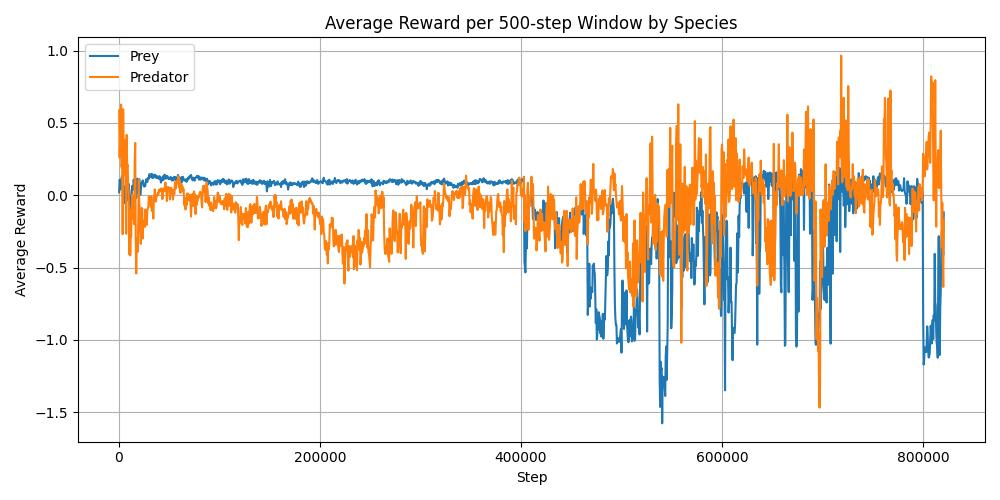
\includegraphics[width=0.9\linewidth]{Bilder/collapse.jpg}
\caption{Policy Collapse bei Jäger und Beute}
\label{fig:reward}
\end{figure}

\section{Diskussion}

Die unzureichenden Lernergebnisse lassen sich auf mehrere kritische Faktoren zurückführen. Die komplexe und wenig differenzierte Reward-Struktur verhinderte klare und konsistente Lernsignale. Widersprüchliche und unklare Belohnungen verwirrten die Agenten und resultierten in ineffizienten Verhaltensmustern.

Darüber hinaus erschwerte die verwendete Zustandsrepräsentation mittels rasterbasierter Beobachtung ohne explizite Positions- oder Richtungsinformationen eine klare und konsistente Interpretation der Umgebung. Die inkonsistente Wahrnehmung, hervorgerufen durch sprunghafte Änderungen der Blickrichtung und kategoriale Kodierung, verstärkte diese Problematik zusätzlich. Zusätzlich verschärften Belohnungskomponenten, die das Annähern an Nahrung oder das Entfernen von Gegnern belohnten, die Problematik. Wenn mehrere Objekte gleichzeitig wahrnehmbar waren, entstanden widersprüchliche Signale. So konnten Bewegungen in verschiedene Richtungen gleichermaßen positiv bewertet werden, was dazu führte, dass die Agenten oft in einem ziellosen Hin-und-Her-Verhalten zwischen zwei relevanten Objekten verharrten, anstatt zielgerichtete Strategien zu entwickeln.

Ein weiterer kritischer Punkt war die getrennte Behandlung von Bewegungs- und Angriffsentscheidungen, die aufgrund der doppelten Aktionsauswahl häufig zu redundanten oder widersprüchlichen Handlungen führte. Diese strukturellen Schwächen verhinderten die Entwicklung robuster und generalisierbarer Strategien.

Zukünftige Untersuchungen sollten daher eine vereinfachte und differenzierte Belohnungsstruktur, eine stabilere und konsistentere Zustandsrepräsentation sowie eine integrierte Aktionsauswahl berücksichtigen, um nachhaltige Lernprozesse zu fördern.

    \chapter{Single-Agenten Methodik}
\label{chap:methodology}
Da die folgenden Versuche alle mit der gleichen Grundmethodik arbeiten, werden alle Gemeinsamkeiten in diesem Kapitel erläutert. Einzelne Details zu den jeweiligen Versuchen folgen in den Methodikabschnitten in Kapitel~\ref{chap:single-tasks}.

\section{Environment}

Die simulierte Umgebung ist modular aufgebaut und stellt eine vereinfachte Überlebenssituation dar, in der unterschiedliche Komponenten je nach Szenario flexibel kombiniert werden können. Die Grundlage bildet eine rechteckige Karte mit kontinuierlich definierten Positionen. Zu den modularen Komponenten zählen rechteckige Nahrungsfelder, welche Nahrungsquellen repräsentieren und von Beute-Agenten genutzt werden können. Diese Felder regenerieren sich langsam bis zu einem festgelegten Maximalwert, wenn sie nicht vollständig geleert wurden. Optional kann ein Fluss als unpassierbare Barriere eingebunden werden, der sowohl Sichtlinien als auch Bewegungswege der Agenten einschränkt. Zusätzlich erhöhen kleine, kreisförmige Hindernisse in Form von Steinen die Navigationskomplexität innerhalb der Umgebung.

Zur Steigerung des Überlebensdrucks existiert außerdem ein Jäger-Agent, der deterministisch nach einer festgelegten Logik handelt. Er verfolgt Beute-Agenten direkt, sofern keine Hindernisse im Weg sind. Sollte die direkte Route blockiert sein, verwendet er den A*-Algorithmus, um heuristisch den kürzesten alternativen Pfad zu finden. Die Geschwindigkeit des Jägers ist bewusst geringer als die der Beute-Agenten, wodurch den Beute-Agenten eine realistische Chance auf Überleben geboten wird. Diese modulare Struktur erlaubt es, Szenarien individuell zu konfigurieren und gezielt unterschiedliche Herausforderungen für die Agenten zu erzeugen.

\section{Observation Space}
Agenten erhalten als Input aus dem Environment drei Kategorien an Inputs. Daten über den eigenen Zustand wie Position, Blickrichtung sowie aktuelle Geschwindigkeit, welche jeweils normalisiert dargestellt werden.
\[
\Bigl[ \,
  \text{ Position }[x,y],\,
  \text{ Blickrichtung }[x,y],\,
  \text{ Geschwindigkeit }[x,y],\,
\Bigr]
\]
Ebenfalls erhalten sie konkrete Informationen über Objekte und Agenten in ihrem Sichtfeld. Hierzu werden in ihrem Sichtfeld Strahlen erzeugt, welche auf Kollisionen prüfen. Der Agent erhält so Winkel, normierte Distanz und Art des Objekts, mit dem der Strahl kollidiert ist, kodiert in One-Hot. Diese Kollisionsarten beinhalten den Rand der Karte, Steine, Flüsse, Jäger-Agenten, sowie Felder und  keine Kollision. Um die Erkennung von Jäger-Agenten zu vereinfachen, wurde für die Strahlenkollision ein Radius um den Agenten weiterhin als Treffer gezählt, auch wenn der Strahl den Agenten nicht direkt getroffen hat. Ist das Objekt ein Feld, wird ebenfalls in Prozent übergeben, wie viel Essen auf dem Feld verfügbar ist. Das Sichtfeld des Beute-Agenten beträgt 180 Grad, während die Länge auf 35 Einheiten (35 Prozent der Kantenlänge der Karte) und die Menge auf 15 Strahlen begrenzt ist. Die folgende Graphik zeigt eine Abbildung der Strahlen, während im Rest der Arbeit für bessere Visualisierung eine vereinfachte Darstellung verwendet wird. 
\begin{figure}[h]
  \centering
  \adjincludegraphics[
     width=0.7\linewidth,
     Clip={0 {0\height} 0 {0.08\height}} 
  ]{Bilder/ray_visual.png}
  \caption{Strahlensensorik}
  \label{fig:ray-observation}
\end{figure}
\newline
Wie in Abbildung~\ref{fig:ray-observation} zu sehen ist, läuft Strahl 1 hier ins leere, und zeigt somit mit maximaler Distanz die in Tabelle~\ref{tab:strahlkomponenten} gezeigte Kodierung „Kein Treffer“. Strahl 2 wiederum trifft bei circa 80 Prozent der Sichtweite auf einen Stein, und kodiert diesen dementsprechend. Im linken Sichtbereich des Agenten befindet sich ein Feld, welches 90 Prozent der Maximalkapazität an Futter enthält. Dieses wird von Strahl 3 mit einer relativen Distanz von circa 0.4 kodiert. Zusätzlich zur Art und Distanz des Objektes wird auch die Richtung kodiert, indem für jeden Strahl die Sinus- und Kosinus-Werte des Winkels relativ zur Blickrichtung des Agenten übergeben werden. Diese Kodierung der Richtung mittels Sinus- und Kosinus-Werten ermöglicht eine kontinuierliche und eindeutige Repräsentation der Winkel, die keine diskreten Sprünge oder Grenzwertprobleme aufweist. Dadurch wird eine stabile und konsistente Verarbeitung durch neuronale Netze gewährleistet, was wiederum zu besseren Generalisierungs- und Lernfähigkeiten beiträgt.
\begin{table}[htbp]
\centering
\caption{Komponenten und Werte für verschiedene Strahlen}
\label{tab:strahlkomponenten}
\begin{tabular}{llll}
\toprule
\textbf{Komponente}        & \textbf{Strahl 1} & \textbf{Strahl 2} & \textbf{Strahl 3}\\
\midrule
Distanz                    & 1.0               & 0.8 & 0.4 \\
sin $\theta$               & $\approx0.90$    & 0   & 1   \\
cos $\theta$               & $\approx0.43$    & 1   & 0   \\
\midrule
\multicolumn{4}{l}{\textbf{One-Hot-Kodierung}}\\
kein Treffer & 1 & 0 & 0\\
Kartenrand      & 0 & 0 & 0\\
Jäger           & 0 & 0 & 0\\
Fluss           & 0 & 0 & 0\\
Stein           & 0 & 1 & 0\\
Feld            & 0 & 0 & 1\\
\midrule
Feldfüllstand & 0.0 & 0.0 & 0.9\\
\bottomrule
\end{tabular}
\end{table}

Die letzte Kategorie an Inputs bilden zwei Supportvektoren. Diese beinhalten jeweils einen Richtungsvektor sowie eine normierte Distanz. Diese Supportvektoren wurden je nach Trainingsszenario angepasst und kodieren unterschiedliche Informationen, welche im weiteren Verlauf weiter besprochen werden.
\[
\bigl[\,
    \text{ Support-Vektor 1 }[x,y],\,
    \text{ Distanz 1},\,
    \text{ Support-Vektor 2 }[x,y],\,
    \text{ Distanz 2}
\bigr]
\]

  
\section{Action Space}
Aufgrund der in Kapitel~\ref{chap:explorative} geschilderten Probleme im Umgang mit konkreten Bewegungsvektoren wurde eine alternative Action-Space-Architektur implementiert. Diese orientiert sich an dem in \cite{baker2020emergenttoolusemultiagent} beschriebenen Ansatz, bei dem Agenten über diskrete Aktionsentscheidungen kontinuierliche Bewegungen steuern.

Die Agenten wählen aus jeweils fünf Aktionen in X- und Y-Richtung sowie drei Aktionen entlang der Z-Achse. In X- und Y-Richtung stehen dabei zwei Impulsstärken in beide Richtungen sowie ein neutraler Impuls zur Verfügung. Die Z-Achse beeinflusst die Rotationsgeschwindigkeit des Agenten, wobei Impulse nach links, rechts oder keine Rotation gesetzt werden können. Aus diesen diskreten Eingaben ergibt sich ein Bewegungsvektor, der über Zeit die Fortbewegung des Agenten bestimmt. Die Beschränkung des Aktionsraums auf eine überschaubare, diskrete Menge ermöglicht stabilere Policy-Updates, da der Agent nur zwischen klar definierten Bewegungsstufen wählen kann. Durch die gewählte Stärke der Impulse sind sowohl größere Schritte als auch kleine Anpassungen möglich. Diese Impulse wirken gemeinsam mit der aktuellen Geschwindigkeit und einer simulierten Reibung auf die Bewegung ein und bestimmen so die neue Position. Dieser Aufbau bietet einen simpleren Action Space, welcher trotzdem zu präzisen und kontinuierlichen Bewegungen führt. 


\section{Netzwerk-Architektur}
Die trainierten Modelle basieren auf einer Actor-Critic-Architektur und verarbeitet zeitliche Abhängigkeiten über ein zweischichtiges LSTM. Die Eingabewerte werden zunächst in eine Dense-Layer gegeben und durch eine Layer-Normalisierung stabilisiert. Anschließend durchlaufen diese normalisierten Vektoren ein LSTM, welches ebenfalls mit Layer-Normalisierung versehen ist. Dieser Output wird dann in 2 verschiedene Heads geteilt. Der Policy-Head und der Value-Head. Der Policy-Head besteht aus 2 weiteren Dense-Schichten, welche die Merkmale für die Aktionsverteilung aufbereiten. Jede der Aktionen erhält hier eine kategoriale Verteilung passend zu der Anzahl an Bins. Aus jeder dieser drei Verteilungen wird eine Aktion gezogen und die logarithmierte Wahrscheinlichkeit für das Policy-Gradient-Update gespeichert. Der Value-Head bereitet in 2 Dense-Schichten die Informationen auf und gibt einen erwarteten kumulierten Value zurück, welcher ebenfalls für das Policy-Gradient-Update dient. Die Aufteilung der Outputs dient der effizienteren Feature-Extraction und stellt sicher, das sich die Aufbereitung der Features auf relevante Abschnitte spezialisieren kann. Diese Kombination gewährleistet, dass das Modell einerseits informierte Aktionsentscheidungen trifft und andererseits zuverlässige Wertschätzungen für eine stabile Policy-Optimierung liefert. Die verwendete Anzahl an Neuronen per Schicht sind in Tabelle ~\ref{tab:neuronenanzahl} aufgelistet.

\begin{table}[htbp]
\centering
\caption{Neuronenanzahl pro Schicht im Netzwerk}
\label{tab:neuronenanzahl}
\begin{tabular}{lc}
\toprule
Schicht & Neuronenanzahl \\
\midrule
Flat Input Dense & 32 \\
Ray Input Dense & 128 \\
Ray Dense & 96 \\
LSTM & 256 \\
Policy Head Dense & 64 \\
Value Head Dense & 32 \\
\bottomrule
\end{tabular}
\end{table}

\section{Training}
Das Training basiert auf dem in Kapitel~\ref{chap:theorie} beschriebenen PPO-Algorithmus. In jedem Simulationsschritt wählt der Agent eine Aktion auf Grundlage seiner aktuellen Beobachtung und des internen LSTM-Zustands. Beobachtung, Aktion, Log-Wahrscheinlichkeit, empfangener Reward sowie der geschätzte Value werden sequentiell im Episodenpuffer abgelegt. Sobald entweder die vordefinierte Sequenzlänge erreicht ist oder eine Terminationsbedingung (beispielsweise Ziel erreicht oder Agent gefressen) eintritt, wird die gesamte Episode gemeinsam mit dem zugehörigen initialen LSTM-Zustand in den Trainingspuffer überführt.

Sobald der Trainingspuffer eine definierte Anzahl von Sequenzen enthält, wird dieser in Mini-batches unterteilt und das Modell durch diese aktualisiert. Dabei werden mehrere PPO-Updates durchgeführt, bei denen sowohl die Policy als auch der Value-Loss berücksichtigt werden. Zwischen den Updates wird der LSTM-Zustand mithilfe der gespeicherten Hidden States initialisiert, um den sequentiellen Kontext zu erhalten. Eine Episode endet für einen Agenten, wenn eine terminierende Bedingung erfüllt ist, zum Beispiel Erreichen des Ziels oder Überschreiten der maximalen Lebenszeit. Danach wird das Environment inklusive aller Agenten zurückgesetzt. Während des Trainings werden Metriken zur späteren Analyse aufgezeichnet, wie beispielsweise  der Gesamtloss, der separate Beitrag des Policy-Losses sowie des Value-Losses. Diese Kennzahlen geben Auskunft darüber, wie gut das Modell aktuelle Strategien und Wertfunktionen approximiert. Zusätzlich wird die mittlere Entropie überwacht, welche die Aktionsunsicherheit des Agenten misst und ein Indikator für das Erkundungsverhalten im Lernprozess ist. Die Gesamtnorm der Gradienten dient als Metrik zur Beurteilung der Trainingsdynamik und erlaubt Rückschlüsse auf die Stabilität und Intensität der Gewichtsaktualisierungen im Modell.

Es wurde ebenfalls ein Learningrate-Scheduler sowie ein Entropy-Scheduler verwendet. Diese Verwenden einen Anfangs höheren Wert für die Lernrate sowie den Entropiekoeffizienten, um zu Beginn durch mehr Exploration und größere Lernschritte effizienter in eine grob Funktionierende Policy zu finden, welche im weiteren Verlauf mit kleineren Lernschritten verfeinert wird.

\begin{table}[htbp] 
    \centering
    \caption{Trainingshyperparameter}
    \label{tab:parameterwerte}
    \begin{tabular}{@{}lcc@{}}
        \toprule
        Parameter & Symbol & Wert\\
        \midrule
        Diskontfaktor & \(\gamma\) & 0.99 \\
        PPO-Clip & \(\epsilon\) & 0.1 \\
        Learning Rate (Start)               & \(\alpha_{\mathrm{start}}\)  & \(1\times10^{-5}\)  \\
        Learning Rate (Ende)                & \(\alpha_{\mathrm{min}}\)    & \(1\times10^{-6}\)  \\
        Environment Steps                   & –                       & 5 000 000  \\
        \bottomrule
    \end{tabular}
\end{table}
Das Training wurde mit verschiedenen Hyperparameter-Konfigurationen getestet, um stabilen Trainingsfortschritt sicherzustellen. Dabei zeigte sich, dass eine niedrige Lernrate sowie enges Clipping wesentlich für die Stabilität sind, da zu große Updates ansonsten Instabilitäten hervorrufen könnten. Tabelle~\ref{tab:parameterwerte} enthält die final verwendeten Hyperparameter, welche nach mehreren Iterationen im Training die stabilsten Ergebnisse lieferten.

Die Tabelle~\ref{tab:data_handling} fasst weitere Parameter zusammen, die das Datenhandling betreffen. Verschiedene Varianten dieser Parameter wurden getestet, wobei die hier dargestellten Werte für das bestehende Environment sowie für die Modellstruktur die besten Trainingserfolge zeigten.

\begin{table}[htbp]
  \centering
  \caption{Datenhandling}
  \label{tab:data_handling}
  \begin{tabular}{ll}
    \toprule
    Parameter             & Wert     \\
    \midrule
    Batch-Größe           & 128       \\
    PPO-Schritte pro Update & 3         \\
    Buffer-Größe          & 512      \\
    Sequenzlänge          & 128      \\
    \bottomrule
  \end{tabular}
\end{table}
    \clearpage{\pagestyle{empty}\cleardoublepage}
    \chapter{Single-Agenten Tasks}
\label{chap:single-tasks}
Um die Auswirkungen verschiedener Trainingsszenarien sowie die jeweils nötigen Anpassungen zu untersuchen, wurden mehrere spezifische Tasks erstellt. Die zentrale Aufgabe des Agenten besteht darin, sein Überleben zu sichern, indem er rechtzeitig eine Futterquelle findet und aufbraucht, bevor er vom Jäger gefangen wird. Diese Aufgabe lässt sich hier in drei einfachere Aufgaben aufteilen. Diese unterscheiden sich im Aufbau der Karte, Rewardfunktion sowie der spezifischen Hilfsvektoren, den sie als Observation erhalten. Die Tasks haben ebenfalls unterschiedliche Terminationsvoraussetzungen für die Trainingsepisoden.

\section{Task 1: Navigation}
\subsection{Methodik}
Task 1 stellt dem Agenten die Aufgabe, zur Position eines bekannten Zielpunkts zu navigieren. Der Agent erhält als Hilfsvektor die Richtung und Distanz zum Zielpunkt, auch wenn dieser sich nicht im Sichtfeld des Agenten befindet. Die Episode endet, wenn der Agent sich innerhalb eines bestimmten Radius vom Ziel befindet. 

\begin{figure}[htbp]
  \centering
  \adjincludegraphics[
     width=0.8\linewidth,
     Clip={0 {0\height} 0 {0.1\height}} 
  ]{Bilder/navigate.png}
  \caption{Navigation}
  \label{fig:navigate_scenario}
\end{figure}

Für das Training des Modells wurden mehrere Parameter und Rewardfunktionen getestet. In der ersten Variante erhielt der Agent eine negative Belohnung für jeden Kontakt mit Wänden und Hindernissen, und eine positive Reward für das annähern an den Zielpunkt. Diese wurde durch die Differenz der Distanz $D_t$ zum Ziel zur Distanz $D_t-1$ zum Ziel im vorherigen Schritt berechnet. In der angepassten Version wurde die Strafe für Wandkollisionen so modifiziert, dass sie mit abnehmendem Abstand zur Wand stärker ausfällt, wodurch ein abrupter Abfall der Belohnung vermieden wird. Ebenfalls wurde die Belohnung für die Distanzänderung zum Ziel so gestaltet, das diese nicht-linear ansteigt. Die letzten Schritte zum Ziel hin beziehungsweise vom Ziel weg sind deutlich wichtiger als eine leichte Justierung in weiter Distanz, und werden deshalb hier stärker gewichtet.

\subsection{Ergebnisse}
Während des Trainings zeigt sich eine stetige Verbesserung der Navigationsfähigkeit des Modells. Wie in Abbildung~\ref{fig:navigation_training_curve} dargestellt, reduziert sich die durchschnittliche Dauer der Episoden, also die benötigte Zeit zum Erreichen des Zielpunkts, über den Verlauf des Trainings. Besonders in den Anfangsphasen des Trainings verbessert sich das Modell deutlich, während sich die Verbesserung nach etwa 5.000 Episoden verlangsamt und sich schließlich einem  Plateau annähert. Dies deutet darauf hin, dass der Agent eine effiziente Strategie zur Zielerreichung erlernt und die relevanten Navigationsfähigkeiten erfolgreich internalisiert.
\begin{figure}[htbp]
\centering
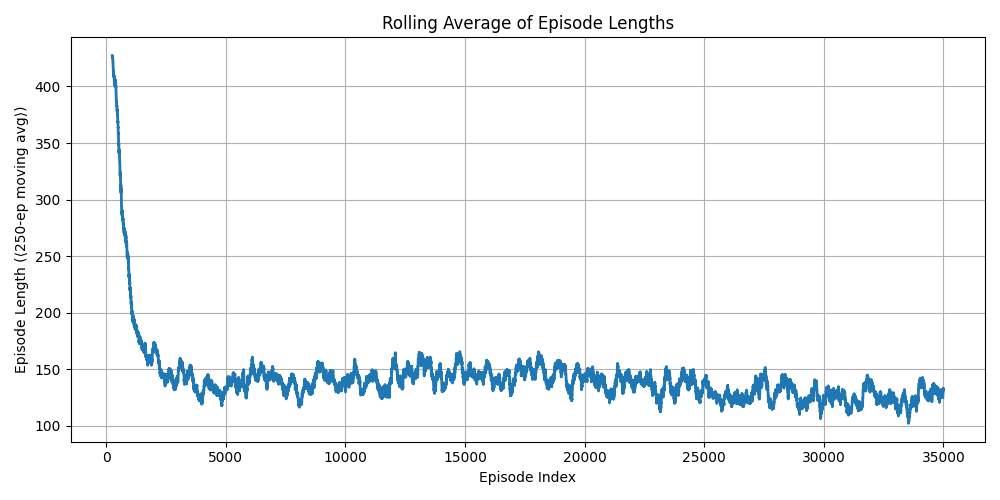
\includegraphics[width=0.9\linewidth]{Bilder/episode_lengths_rolling.png}
\caption{Mittlere Episodenlänge pro 250 Epochen – Navigation}
\label{fig:navigation_training_curve}
\end{figure}
\subsection{Diskussion}
Das Training im Navigationstask verlief insgesamt stabil und führte zu klaren Fortschritten beim Erlernen einer zielgerichteten Bewegung. Dies liegt unter anderem an der kontinuierlichen und dichten Rewardfunktion, die dem Agenten in jeder Situation ein verwertbares Feedback bietet. Besonders die nicht-lineare Skalierung der Belohnung in Zielnähe erwies sich als hilfreich, da sie das Modell dazu motivierte, auch die letzten Schritte präzise zu planen.

Eine weitere wichtige Anpassung war die Modifikation der Kollisionsstrafe: Anstatt harter Bestrafungen bei Kollisionen wurde eine kontinuierliche Penalty eingeführt, die stärker wird, je näher sich der Agent an eine Wand bewegt. Dies reduzierte deutlich die Zahl der Wandkollisionen im Verhalten des Agenten. Allerdings schlägt sich dieser Effekt kaum bis gar nicht in den aggregierten Metriken nieder – etwa weil die Anzahl der Kollisionen keinen direkten Einfluss auf die Episodendauer hat oder durch andere Lernfortschritte überdeckt wird.

Die klare Zielstruktur und die stets verfügbaren Hilfsvektoren (Richtung und Distanz zum Ziel) ermöglichen ein vergleichsweise einfaches Lernen. Allerdings schränkt diese künstliche Unterstützung die Generalisierbarkeit ein – in realitätsnäheren Szenarien wären solche Informationen möglicherweise nicht direkt zugänglich. Eine potenzielle Erweiterung wäre daher, das Training auf rein visuelle Eingaben zu beschränken oder einen gestaffelten Zugriff auf Zielinformationen einzuführen.

\section{Task 2: Exploration}
\label{sec:explore}
\subsection{Methodik}
Task 2 enthält nur eine Futterquelle auf der Karte. Ziel des Agenten ist es, über die leere Karte zu laufen, um das Feld zu finden und es anschließend zu leeren. Der Hilfsvektor ist in dieser Aufgabe nur aktiv, wenn der Agent das Feld im Sichtfeld hat, oder der Agent sich innerhalb eines festgelegten Abstands vom Feld aufhält. Für das Training des Exploretasks wurden iterativ mehrere Modelle mit verschiedenen Rewardfunktionen trainiert.
\begin{figure}[htbp]
  \centering
  \adjincludegraphics[
     width=0.9\linewidth,
     Clip={0 {0\height} 0 {0.1\height}} 
  ]{Bilder/explore.png}
  \caption{Exploration}
  \label{fig:explore_scenario}
\end{figure}

\subsection{Varianten}
\begin{table}[h]
  \centering
  \caption{Reward-Varianten im Explore-Task}
  \begin{tabular}{@{}lll@{}}
    \toprule
    Kürzel & Besondere Reward-Komponente & Motivation \\ \midrule
    V1 & $\Delta$ Distanz zum Feld + gesammeltes Futter & Bewegung zum Feld  \\
    V2 & $\Delta$ Distanz zum Feld wenn in Sicht + Futter & Vermeidung irrelevanter Signale\\
    V3 & V2 + Shaping für Erkundung      & Sparse-Reward-Problem  \\ 
    V4 & V3 mit angepassten Shaping-Parameterm & Optimierung
    \\ \bottomrule
  \end{tabular}
\end{table}

Die ersten Modelle wurden für das verringern der Distanz zum Feld belohnt. Hierbei wurde die Differenz der Distanz $D_t$ zum Feld zur Distanz $D_t-1$ verwendet. Ebenfalls erhält der Agent eine Belohnung, wenn Futter gesammelt wird, er sich also auf dem Feld befindet. In Variante 2 wird die Distanzreward nur gegeben, wenn der Agent das Feld im Sichtfeld hat oder sich innerhalb eines Mindestabstands vom Feld aufhält. In Variante 3 wurde zusätzlich zur Reward in Variante 2 eine Belohnung für das Erkunden der Karte gegeben. Hierbei wurde die Karte in Unterabschnitte unterteilt und der Agent für das Besuchen jedes Kartenabschnittes belohnt. Die Reward auf jedem Unterabschnitt nimmt exponentiell ab, bis sie nach einer bestimmten Anzahl an Schritten auf dem Feld eine linear steigende negative Reward gibt. Dies soll dazu führen, dass der Agent mehrere Felder abläuft, auf diesen aber nicht zu lange verweilt. Für das Training mit Variante 4 wurden die Parameter der Explorationsreward angepasst, indem die Größe der Unterabschnitte variiert wurde. Dies sollte das Erkunden der Karte weiter anregen.

\subsection{Ergebnisse}
\begin{figure}[htbp]
  \centering
  \adjincludegraphics[
     width=0.8\linewidth,
     Clip={0 {0\height} 0 {0.06\height}} 
  ]{Bilder/explore_comparison.jpg}
  \caption{Trainingsverlauf nach Rewardfunktion - Exploration}
  \label{fig:normalized_learning_curves_explore}
\end{figure}
Abbildung ~\ref{fig:normalized_learning_curves_explore} zeigt die normalisierten Rewards während des Trainings der jeweiligen Modelle. \emph{windowed} zeigt dabei jeweils die über Fenster von 25.000 Schritten gemittelten und anschließend normalisierten Rewards. \emph{trend} verwendet über 11 dieser Werte einen gleitenden Durchschnitt, um eine geglättete Trendkurve zu zeigen. Das mit Variante 1 trainierte Modell zeigt direkt anfangs eine kleine Verbesserung, landet danach allerdings in einem Plateau und zeigt keine weitere Verbesserung. Variante 2 zeigt zunächst eine vergleichbare Leistungssteigerung wie Variante 3 und 4, stagniert jedoch frühzeitig und weist im weiteren Verlauf sogar eine systematische Verschlechterung auf. Der Trainingsverlauf geht zum Ende des Trainings wieder leicht nach oben, liegt aber immer noch weiter unter der Performance von Varianten 3 und 4. Diese beiden Modelle zeigen ähnliche Lernkurven, bei denen beide zunächst starke Verbesserungen zeigen, und danach weiter langsam die Ergebnisse stabil verbessern. Die Endperformance von Variante 4 übertrifft die von Variante 3 leicht. Zwar zeigte letztere zu Beginn des Trainings schnellere Fortschritte, diese flachten im weiteren Verlauf jedoch deutlich ab, sodass sie letztlich geringfügig hinter der Nachfolgevariante zurückbleibt.

\subsection{Diskussion}
Das Training im Explore-Task zeigte sich sehr instabil, was letztlich auch zu einer insgesamt schwachen Performance führte. Trotz verschiedener Rewardvarianten konnte kein Modell konsistent lernen das Feld zuverlässig zu finden und zu leeren. Hauptgrund dafür ist die starke Sparsity des Rewards: Belohnung wird nur bei Sichtkontakt oder direkter Nähe zum Feld erteilt – ein Zustand, der ohne zusätzliche Struktur selten eintritt.

Ergänzende Shapingkomponenten wie weitere Erkundungsbelohnungen oder das Belohnen der ersten Sichtung des Felden zeigten nur begrenzte Wirkung. Der Agent blieb häufig entweder vollkommen stehen und lief nur auf zufällig nahegelegene Felder, oder rannte mit voller Geschwindigkeit über die Karte und ignorierte die Felder vollständig. Dies zeigt deutlich, das der Agent die Aufgabenteilung \emph{Feld finden} und \emph{Feld leeren} nur kaum vereinbaren konnte.

Eine sinnvolle Weiterentwicklung wäre der Einsatz von intrinsischer Motivation (zum Beispiel durch curiosity-driven learning) oder hierarchischen Policies, bei denen ein übergeordneter Agent Explorationsziele vorgibt. Zudem wäre eine alternative Evaluation sinnvoll, etwa die Erfolgsdefinition über das erstmalige Erreichen des Feldes, statt über das vollständige Leeren.

\section{Task 3: Fleeing}
\label{sec:flee}
\subsection{Methodik}
Task 3 beinhaltet neben ein paar Hindernissen einen Jäger-Agenten, der gezielt auf den Beute-Agenten zusteuert. Ziel des Agenten ist es, dem Jäger so lange wie möglich zu entkommen. Belohnt wird hier das Vergrößern der Distanz zum Jäger sowie die bisher überlebte Zeit. Die Belohnung wird bewusst verzögert aktiviert, um passives Verhalten zu Beginn der Episode zu vermeiden. Da der Jäger initial in einer bestimmten Entfernung erscheint, würde eine sofortige Überlebensbelohnung dazu führen, dass der Agent ohne aktives Ausweichverhalten belohnt wird. Nach dieser Verzögerung steigt die Überlebensbelohnung langsam bis zu einem Schwellwert an. Als Hilfsvektor erhält der Agent hier die Richtung sowie die Distanz zum Jäger. Mehrere Varianten der Umgebungskonfiguration wurden getestet, darunter Szenarien mit und ohne Fluss sowie mit unterschiedlich großen Hindernissen. Zum Vergleich dieser Einstellungen wurden jeweils separate Modelle trainiert und anschließend evaluiert.
\begin{figure}[htbp]
  \centering
  \adjincludegraphics[
     width=0.9\linewidth,
     Clip={0 {0\height} 0 {0.1\height}} 
  ]{Bilder/flee.png}
  \caption{Flucht}
  \label{fig:flee_scenario}
\end{figure}
\subsection{Ergebnisse}
Abbildung \ref{fig:episode_lengths} zeigt den Mittelwert der Episodenlängen über den Trainingsverlauf der Modelle, die mit unterschiedlichen Hindernissen trainiert wurden. Es ist zu erkennen, dass alle drei Modelle im Laufe des Trainings zunehmend länger überleben, indem sie dem Jäger effektiver entkommen. In den Graphen treten mehrfach temporäre Plateaus auf, die nach weiterem Training jedoch jeweils wieder überwunden werden. Gegen Ende des Trainings liegen die Überlebensdauern des „Medium Rocks“- und des „River“-Modells auf ähnlichem Niveau, während das „Big Rocks“-Modell eine deutlich höhere durchschnittliche Episodenlänge erreicht.

Dabei ist zu beachten, dass die Schwierigkeit der Szenarien unterschiedlich ausfällt, da sie stark von der Navigationslogik des Jägers abhängt: Schon zu Beginn des Trainings weist das River-Szenario eine höhere Überlebensdauer auf, weil der Jäger eine größere Distanz überwinden muss. Trotzdem fällt die Verbesserung gegenüber der Baseline beim River-Modell sehr gering aus und bleibt insgesamt auf niedrigerem Niveau. Im Gegensatz dazu starten beide Fels-Szenarien (mittelgroße vs. große Hindernisse) mit ähnlich niedrigen Baselines, zeigen nachfolgend jedoch einen deutlich stärkeren Leistungszuwachs.
\begin{figure}[htbp]
  \centering
  \adjincludegraphics[
     width=0.8\linewidth,
  ]{Bilder/ep_lengths.jpg}
  \caption{Mittlere Episodenlänge pro 250 Epochen – Flucht}
  \label{fig:episode_lengths}
\end{figure}

Um die Performance der Modelle unabhängiger testen zu können, wurden diese in einem einheitlichen Environment erneut getestet. Dieses Environment enthält sowohl einen Fluss als auch mehrere kleine Steine, was dem Hindernissaufbaue des Survival-Tasks (\ref{sec:survival}) entspricht. Die Tabelle~\ref{tab:survival_comparison} zeigt die durchschnittliche Überlebensdauer der jeweiligen Modelle, berechnet über 1000 Episoden in der beschriebenen Umgebung. Hierbei zeigt sich, dass das Modell aus dem Fluss-Szenario schlechter abschneidet, obwohl dieses dem getesteten Aufbau ähnlicher ist als die anderen beiden Environments. Das „Medium Rocks“-Modell zeigt hierbei die beste Performance, während die Leistung des „Big Rocks“-Modells leicht unter der des „River“-Modells liegt.

\begin{table}[h]
  \centering
  \caption{Überlebensdauer im Survival-Task}
  \begin{tabular}{@{}l c@{}}
    \toprule
    Trainingsszenario &
      \multicolumn{1}{c}{durchschnittliche Überlebensdauer} \\ \midrule
    große Steine   & $71,6 \pm 1,5$ \\
    mittelgroße Steine  & $89,4 \pm 2,1$ \\
    Fluss          & $78,4 \pm 1,8$ \\ 
    \bottomrule
  \end{tabular}
  \label{tab:survival_comparison}
\end{table}


\subsection{Diskussion}
Die Ergebnisse aus Tabelle \ref{tab:survival_comparison} verdeutlichen, dass die Übertragbarkeit der Subtask-Modelle in das einheitliche Test-Environment nicht allein durch die strukturelle Ähnlichkeit des Trainingsszenarios erklärt werden kann. Obwohl das River-Modell dem Aufbau der Testumgebung am ähnlichsten ist, erreicht es eine geringere Überlebensdauer als die des Modells, welches mit kleinen Hindernissen trainiert wurde. Dies deutet darauf hin, dass der erhöhte Abstand zum Jäger im Fluss-Szenario zwar initial das Überleben erleichtert, aber keine robusten Ausweichstrategien fördert. 

Im Gegensatz dazu mussten die Agenten im „Medium Rocks“-Szenario von Beginn an komplexere Routen um Hindernisse planen und adaptiv auf enge Passagen reagieren. Diese stärkere Navigationsanforderung scheint zu allgemeineren und effizienteren Taktiken geführt zu haben, die sich auch im neuen Environment bewähren. 

Die unterschiedlichen Schwierigkeitsgrade der Trainingsszenarien können die absoluten Überlebenszeiten verzerren. Entscheidend ist jedoch, dass das „Medium Rocks“-Modell, trotz des anspruchsvolleren Settings, am stärksten von seinem Training profitiert und die höchsten Überlebenswerte erzielt. Insgesamt legt dies nahe, dass eine höhere Komplexität im Subtask-Training hier die Generalisierungsfähigkeit verbessert und zu nachhaltigeren Fluchtstrategien führt.


\section{Task 4: Survival}
\label{sec:survival}
\subsection{Methodik}
Dieser Task beschreibt das eigentliche Endziel, welches das Modell erreichen soll. In diesem Environment hat der Agent die Aufgabe, eine Futterquelle zu finden und zu leeren, bevor er vom Jäger gefressen wird. Er erhält als Hilfsvektoren sowohl die Richtung und Distanz zum Jäger, als auch die Richtung und Distanz zum Feldstück, wenn er dieses in seinem Sichtfeld hat. 
\begin{figure}[htbp]
  \centering
  \adjincludegraphics[
     width=0.9\linewidth,
     Clip={0 {0\height} 0 {0.1\height}} 
  ]{Bilder/full.png}
  \caption{Gesamtszenario}
  \label{fig:full_scenario}
\end{figure}
Da dieses Szenario Komponenten all der Unteraufgaben enthält, wurde zunächst eine Kombination der drei taskspezifischen Rewardfunktionen getestet. Diese Rewardfunktion belohnte somit das Verkleinern der Distanz von sichtbaren Feldabschnitten, das Vergrößern der Distanz zum Jäger, das Vermeiden von Kollisionen, sowie eine Belohnung für längeres Überleben und eine Strafe für eine Kollision mit dem Jäger. Ebenfalls wurde die zeitverzögerte Überlebensbelohnung aus dem Abschnitt~\ref{sec:flee} übernommen. Es wurde ebenfalls eine vereinfachte Rewardfunktion implementiert, um das Training zu stabilisieren und gegenläufige Signale zu vermeiden.

Diese angepasste Rewardfunktion entfernt die gegenläufige Überlebensbelohnung sowie die Penalty für Kollisionen mit Wänden. Ebenfalls fällt die rasterbasierte Erkundungsbelohnung aus Abschnitt~\ref{sec:explore} weg. Somit bleiben eine Penalty für eine Kollision mit dem Jäger und verstrichene Zeit, sowie Belohnungen für das Vergrößern der Distanz zum Jäger, Verringern der Distanz zu sichtbaren Futterquellen sowie das Sammeln von Futter. Um die Änderungen zu kompensieren, wurden die Parameter der bleibenden Rewardkomponenten leicht angepasst.

\subsection{Ergebnisse}
Abbildung ~\ref{fig:task4_learning_curve} zeigt zwei Trainingsabläufe im vollen Environment. Die Modelle wurden jeweils mit den gleichen Parametern, aber unterschiedlichen Rewardfunktionen trainiert. \emph{combined} zeigt hierbei das Modell, welches mit der Kombination der Rewardfunktionen aus den Subtasks trainiert wurde, während \emph{adjusted} die in der Methodik angepasste und vereinfachte Rewardfunktion verwendet. \emph{windowed} zeigt dabei jeweils die über Fenster von 25.000 Schritten gemittelten und anschließend normalisierten Rewards. \emph{trend} verwendet über 11 dieser Werte einen gleitenden Durchschnitt, um eine geglättete Trendkurve zu zeigen. Die kombinierte Rewardfunktion zeigt insgesamt kaum bis gar keinen Lerneffekt, während sich die Performance des Modells mit justierter Rewardfunktion bis Schritt 2.000.000 verbessert, und danach nur leichte Schwankungen zeigt.

\begin{figure}[htbp]
  \centering
  \adjincludegraphics[
     width=0.8\linewidth,
     Clip={0 {0\height} 0 {0.06\height}} 
  ]{Bilder/learning_curves_task4.png}
  \caption{Trainingsverlauf Surival-Task}
  \label{fig:task4_learning_curve}
\end{figure}
\subsection{Diskussion}
Die Überlebensumgebung stellte sich als besonders herausfordernd heraus, da sie mehrere konkurrierende Ziele gleichzeitig verlangt: Nahrung sammeln, Jäger meiden, Karte erkunden und Hindernisse umgehen. Das initiale Rewarddesign, welches die Rewardfunktionen der Subtasks kombinierte, führte hierbei zu instabilen Lernverläufen. Insbesondere widersprüchliche Signale – etwa Überlebensbelohnung bei gleichzeitigem Ignorieren von Nahrung – verhinderten eine kohärente Strategieentwicklung.

Die vereinfachte Rewardfunktion reduzierte diese Konflikte, was sich in einer deutlich verbesserten Lernkurve widerspiegelte. Hierbei zeigte sich, dass klare, priorisierte Ziele (beispielsweise Nahrungssuche und Flucht mit klaren Bedingungen) besser vom Modell internalisiert werden als komplexe, gleichgewichtete Rewardmischungen. Diese Erkenntnis unterstreicht die Bedeutung einer sorgfältigen Rewardabstimmung bei Multi-Ziel-Szenarien.

\section{Curriculum Learning}
\subsection{Methodik}
\label{sec:methodology}
Der methodische Aufbau zur Untersuchung des Curriculum-Learning-Ansatzes basiert auf dem Vergleich unterschiedlicher Trainingsstrategien. Curriculum Learning bezeichnet eine Strategie, bei der das Training komplexer Modelle schrittweise anhand von zunehmend anspruchsvolleren Aufgaben durchgeführt wird, beginnend mit einfachen Teilaufgaben und schrittweise übergehend in komplexere Szenarien. Konkret wurde hierzu der Trainingsverlauf eines vollständig neu initialisierten Modells mit den Verläufen der Modelle verglichen, deren Gewichte zuvor in den spezifischen Subtasks (Navigation, Exploration, Fleeing) vortrainiert worden waren.

Dazu wurden die jeweils besten Modelle aus den vorhergehenden Subtasks nach dem initialen Training erneut geladen und anschließend im Überlebensszenario weitertrainiert. Ziel dieses Vorgehens war es, zu untersuchen, ob durch das Vortrainieren in vereinfachten Umgebungen eine schnellere Konvergenz oder eine verbesserte finale Performance in der komplexen Gesamtumgebung erzielt werden kann. 

Durch den direkten Vergleich der Lernkurven zwischen neu initialisierten und vortrainierten Modellen konnte somit evaluiert werden, ob der Curriculum-Learning-Ansatz zu signifikanten Vorteilen hinsichtlich der Lerngeschwindigkeit und Qualität der gelernten Strategien führt.\subsubsection*{Bezeichnungen der Modellklassen}
Im Folgenden werden vier Modellklassen unterschieden:
\begin{itemize}
  \item Modelle, die im Navigation-Task vortrainiert und anschließend in der vollständigen Umgebung weiter trainiert wurden, werden \emph{Navigationsmodelle} genannt.
  \item Modelle, die im Exploration-Task vortrainiert und anschließend in der vollständigen Umgebung weiter trainiert wurden, werden \emph{Explorationsmodelle} genannt.
  \item Modelle, die im Fleeing-Task vortrainiert und anschließend in der vollständigen Umgebung weiter trainiert wurden, werden \emph{Fluchtmodelle} genannt.
  \item Frisch initialisierte Modelle, die ohne Vortraining direkt in der Zielumgebung trainiert werden, werden \emph{Scratch-Modelle} genannt.
\end{itemize}
Die Scratch-Modelle besitzen keine vortrainierten Gewichte und werden ausschließlich im vollständigen Szenario von Grund auf trainiert.  

Um dabei einen fairen Vergleich der Trainingsabläufe zu gewährleisten, wurden beim Transfertraining ausschließlich die Modellgewichte geladen, der Optimizer jedoch neu initialisiert. Dies stellt sicher, dass alle getesteten Modelle die gleiche Ausgangsbasis hinsichtlich der Lernrate und weiterer Optimizer-spezifischer Parameter besitzen.


\subsubsection{Evaluierung}
Die Evaluierung der Performance im Environment erfolgte mithilfe mehrerer speziell definierter Metriken. Wichtig sind hierbei unter anderen die Menge des gesammelten Futters, die durchschnittliche Überlebensdauer sowie die durchschnittliche Zeit bis zum vollständigen Leeren eines Feldes.

Bei der Berechnung der jeweiligen Metriken werden nur jene Episoden berücksichtigt, die die entsprechende Voraussetzung erfüllen. Konkret bedeutet dies, dass Episoden, in denen der Agent vom Jäger gefressen wird, ausschließlich zur Ermittlung der durchschnittlichen Überlebensdauer herangezogen werden. Episoden, die erfolgreich mit einem vollständig geleerten Feld enden, werden hingegen für die Berechnung der Zeit-zu-Futter-Metrik genutzt.
 
Diese Aufteilung spielt ebenfalls eine Rolle bei der Berechnung der Erfolgsrate. Als erfolgreich gelten Episoden, in denen der Agent das Feld vollständig leert. Alle anderen Episoden werden als gescheitert gewertet. Die Erfolgsrate gibt somit den Anteil erfolgreicher Episoden an der Gesamtzahl der Evaluierungsepisoden in Prozent an.

Um diese Metriken zu ermitteln, absolvieren jeweils alle drei Modelle aus den vier Gruppen insgesamt 1000 Episoden im Überlebensszenario. Diese Episoden sind für alle Modelle identisch und wurden von keinem der Modelle während des Trainings zuvor gesehen. Die daraus resultierenden Werte werden anschließend gruppenweise zusammengefasst und ausgewertet.

\subsection{Ergebnisse}
\subsubsection{Trainingsverlauf}
Abbildung~\ref{fig:normalized_rewards} zeigt die Trainingsverläufe der in den Subtasks vortrainierten Modelle im Vergleich zum Scratch-Modell. Die dargestellten Werte entsprechen jeweils den Mittelwerten aus drei Trainingsdurchläufen.
\begin{figure}[htbp]
  \centering
  \adjincludegraphics[
     width=0.9\linewidth
  ]{Bilder/learning_curves.png}
  \caption{Trainingsverlauf Curriculum Learning}
  \label{fig:normalized_rewards}
\end{figure}
Zu Beginn des Trainings zeigen die Scratch-Modelle eine schnelle Verbesserung der Performance, erreichen jedoch nach ungefähr der Hälfte des Trainingsverlaufs ein Plateau, auf welchem sich die Leistung nur geringfügig weiter verbessert.

Im Vergleich dazu weisen die Fluchtmodelle eine deutlich flachere Lernkurve auf, was darauf hindeutet, dass diese Modelle zunächst Schwierigkeiten hatten, zusätzliche relevante Strategien (wie das Sammeln von Futter) zu integrieren, nachdem sie zuvor hauptsächlich auf Fluchtstrategien trainiert wurden. Trotz ihres langsameren Fortschritts erreichen die Fluchtmodelle am Ende des Trainings ein ähnliches Performance-Niveau wie die Scratch-Modelle.

Die Navigationsmodelle starten hingegen mit einem deutlich höheren Grundniveau, was darauf hinweist, dass diese bereits relevante Fähigkeiten zur Orientierung und Zielnavigation internalisiert haben. Nach einer schnellen anfänglichen Anpassungsphase erreichen diese Modelle jedoch ebenfalls ein ähnliches Plateau wie die zufällig initialisierten Modelle.

Die Explorationsmodelle zeigen zunächst eine instabilere und insgesamt niedrigere Lernkurve. Allerdings übertreffen diese gegen Ende des Trainingszeitraums leicht die Performance der anderen Modelle. Dies deutet darauf hin, dass die explorativen Fähigkeiten erst im späteren Trainingsverlauf einen Vorteil bieten, nachdem die Agenten gelernt haben, diese Fähigkeiten effizient in die Gesamtstrategie zu integrieren.


\subsubsection{Performance}
Obwohl die Modelle hinsichtlich der Gesamtbelohnung am Ende des Trainings ähnliche Niveaus erreichen, erfasst dieser Wert nicht vollständig alle relevanten Aspekte des Agentenverhaltens. Da die eingesetzte Rewardfunktion unterschiedliche Verhaltensweisen gleichzeitig belohnt, kann ein ähnlich hohes Gesamtrewardniveau unterschiedliche Strategien verschleiern, welche die Modelle jeweils bevorzugen. Um eine differenzierte Bewertung der Performance zu ermöglichen, ist es deshalb notwendig, einzelne Komponenten des Verhaltens separat zu analysieren.
\begin{figure}[htbp]
  \centering
  \adjincludegraphics[
     width=0.6\linewidth
  ]{Bilder/total_food_collected_bar_median.png}
  \caption{Futter pro Episode (median)}
  \label{fig:food_per_episode}
\end{figure}
Abbildung~\ref{fig:food_per_episode} zeigt den Median der Menge an Futter, welches die jeweiligen Modelle in der im Methodikabschnitt ~\ref{sec:methodology} beschriebenen Evaluation gesammelt haben \footnote{Der Median wird aufgrund der hohen Zahl an Ausreißern im Fluchtmodell verwendet, die durch das Nachwachsen des Futters entsteht. Der Agent sammelt so zwar mehr Futter, was aber nicht zwangsläufig zum besseren erfüllen der Aufgabe führt}. Hierbei zeigt sich eine positive Tendenz für die Explorationsmodelle, was sich mit den Erkenntnissen der Trainingsverläufe deckt. Ebenfalls zeigen die Scratch-Modelle insgesamt die schlechteste Performance, während Navigations- und Fluchtmodelle ähnliche Werte aufweisen. Insgesamt zeigen jedoch alle Modelle ähnliche Performance in diesem Bereich.
\newpage

Ebenfalls relevant zu dieser Metrik ist die Betrachtung der Zeit die ein Agent benötigt, um das Feld vollständig zu leeren - ein Agent kann das Feld nach 10 oder nach 100 Schritten vollständig leeren und die gleiche Menge an Futter erhalten.
\begin{figure}[htbp]
  \centering
  \adjincludegraphics[
     width=0.6\linewidth
  ]{Bilder/time_to_goal_bar_se.png}
  \caption{Zeit zu geleertem Feld}
  \label{fig:time_to_goal}
\end{figure}
Hierbei zeigt sich deutlich, dass die Fluchtmodelle länger als die anderen Modelle brauchen, um das Feld zu erreichen und dieses zu leeren. Die Navigations-, Explorations- und Scratch-Modelle zeigen hierbei eine ähnliche Leistung auf.

Episoden, in denen das Feld nicht geleert wurde, fallen stattdessen in die Metrik zur Lebensdauer der Agenten, welche in Abbildung~\ref{fig:time_alive} zu sehen ist.
\begin{figure}[htbp]
  \centering
  \adjincludegraphics[
     width=0.7\linewidth
  ]{Bilder/time_alive_bar_se.png}
  \caption{Lebensdauer}
  \label{fig:time_alive}
\end{figure}
Hierbei zeigt sich eine ähnliche Tendenz zu der in Abbildung~\ref{fig:time_to_goal}, wobei Fluchtmodelle länger überleben. Die anderen Modellarten zeigen hierbei wieder ähnliche Performance, während die Scratch-Modelle hier eine leicht geringere Überlebensdauer aufweisen.

Um die vorherigen beiden Metriken jedoch korrekt einordnen zu können ist ebenfalls die Betrachtung der Erfolgsrate nötig. In der Regel endet eine Episode, weil entweder das gesamte Feld geleert wurde oder weil der Agent von einem Jäger getroffen wurde. Theoretisch existiert noch ein dritter Fall, bei dem keine dieser beiden Bedingungen zutrifft und die Episode durch Erreichen der maximalen Episodenlänge beendet wird. Dieser Fall tritt jedoch sehr selten auf und wurde daher in den bisherigen Metriken der Kategorie Überlebensdauer zugeordnet.

In Abbildung~\ref{fig:succesrate} zählen alle Episoden, die mit einem geleerten Feld enden, als erfolgreich beendet, während alle anderen Episoden als gescheitert gelten. Hier wird deutlich, dass die Explorationsmodelle die beste Leistung besitzen. Die Navigationsmodelle zeigen ebenfalls eine kleine Verbesserung gegenüber den Scratch-Modellen auf, während die Fluchtmodelle schlechter abschneiden. Diese Diskrepanz zu den gesammelten Futterwerten, die in Abbildung~\ref{fig:food_per_episode} gezeigt werden, entsteht durch das Implementierte nachwachsen des Futters. Die Agenten sammeln also alle grob die gleiche Menge an Futter, allerdings scheinen die Explorationsmodelle gezielter auf dem Feld zu warten und es vollständig zu leeren, während die Fluchtmodelle dieses zwar betreten, es allerdings auch schnell wieder verlassen um gegebenenfalls später zurückzukehren. Somit ergibt sich eine ähnliche Menge an gesammeltem Futter mit unterschiedlicher Erfolgsrate.

\begin{figure}[htbp]
  \centering
  \adjincludegraphics[
     width=0.6\linewidth
  ]{Bilder/successful_comparison.png}
  \caption{Anteil erfolgreich beendeter Episoden}
  \label{fig:succesrate}
\end{figure}
\subsection{Diskussion}

Die Evaluation des Curriculum-Learning-Ansatzes zeigte, dass vortrainierte Modelle nicht nur schneller lernen, sondern auch spezialisierte Verhaltensweisen beibehalten – mit teils positiven, teils negativen Folgen. Besonders die Navigationsmodelle profitierten stark vom Vortraining, indem sie zu Beginn schneller das Zielverhalten lernten. Die Explorationsmodelle zeigten erst später Vorteile, entwickelten jedoch eine höhere Erfolgsrate. Dagegen hatten die Fluchtmodelle Schwierigkeiten, ihr Fluchtverhalten mit der Nahrungssuche zu kombinieren, was auf negative Interferenz hinweist.

Diese Beobachtungen zeigen, dass Transferlernen nicht nur Vorteile bringt, sondern auch bestehende Verhaltensmuster verfestigen kann, die im neuen Kontext suboptimal sind. Denkbar wäre hier ein modularer Aufbau der Policy – etwa durch getrennte Komponenten für Flucht und Nahrung, die situativ gewichtet werden.

\section{Retention nach Full-Task-Fine-Tuning}
Im folgenden Abschnitt wird die Performance der Flucht-, Navigations- und Explorationsmodelle im ursprünglichen Subtask mit der Performance der Baseline-Modelle verglichen. Ziel ist es, zu evaluieren, ob die Modelle die ursprünglich gelernten Fähigkeiten nach dem Full-Task-Fine-Tuning beibehalten haben oder ob diese durch neue Strategien ersetzt beziehungsweise abgeschwächt wurden.

\subsection{Methodik}
Für jeden der drei Subtasks—Explore, Flee und Navigate—wurden zwei Modellvarianten jeweils über 1000 unabhängige Episoden hinweg evaluiert. Die Baseline-Modelle wurden ausschließlich im jeweiligen Subtask trainiert, während die Fine-Tuned-Varianten im Anschluss ein zusätzliches Full-Task-Training erhielten. Als Leistungskennzahlen dienten im Explore-Subtask die durchschnittliche Zeit bis zum Erreichen des Ziels (Time to Goal) und die Erfolgsrate (Success Rate), im Flee-Subtask die mittlere Überlebenszeit in Schritten (Time Alive) und im Navigate-Subtask sowohl die Time-to-Goal als auch die Clear Rate, definiert als Anteil der Episoden, in denen das Ziel erreicht wurde.

\subsection{Ergebnisse}

\paragraph{Explore}
Nach dem Full-Task-Fine-Tuning zeigt das Explore-Modell eine deutliche Leistungssteigerung.  
Die durchschnittliche \emph{Time-to-Goal} verkürzt sich von $115{,}8 \pm 3{,}5$ auf $104{,}5 \pm 3{,}0$ Schritte\footnote{Angaben jeweils Mittelwert $\pm$ Standardfehler des Mittelwerts.}. Gleichzeitig steigt die Erfolgsrate um fast dreizehn Prozentpunkte auf $94{,}6\%$. Hier ist zu beobachten, dass der Agent die Futterquellen nicht nur schneller findet, sondern diese auch konsistenter vollständig leert. 

\begin{table}[H]
  \centering\footnotesize
  \setlength{\tabcolsep}{4pt}
  \caption{Retention im Explore-Subtask}
  \begin{tabular}{@{}lcc@{}}
    \toprule
    Modell                     & Time to Goal & Success Rate \\
                               & [Steps]      & [\%]         \\ 
    \midrule
    Explore-only               & $115{,}8 \pm 3{,}5$ & $81{,}7$  \\
    Explore \(\rightarrow\) Survival & $104{,}5 \pm 3{,}0$ & $94{,}6$  \\
    \bottomrule
  \end{tabular}
\end{table}

\paragraph{Flee}
Im Flee-Subtask sinkt die mittlere Überlebenszeit und damit die Performance nach dem Full-Task-Training von $149{,}4 \pm 20$ auf $115{,}1 \pm 2{,}6$ Schritte. 
\begin{table}[H]
  \centering\footnotesize
  \setlength{\tabcolsep}{4pt}
  \caption{Retention im Flee-Subtask}
  \begin{tabular}{@{}lc@{}}
    \toprule
    Modell                     & Time Alive  \\ 
                                & [Steps]   \\ 
    \midrule
    Flee-only                  & $149{,}4 \pm 3{,}3$    \\
    Flee \(\rightarrow\) Survival    & $115{,}1 \pm 2{,}6$  \\
    \bottomrule
  \end{tabular}
\end{table}

\paragraph{Navigate}
Die Time-to-Goal im Navigate-Subtask ist relativ stabil und steigt nach dem Survival-Fine-Tuning von $139 \pm 3{,}3$ auf $142{,}1 \pm 3{,}7$ Schritte, während die Clear Rate wiederum von $95{,}5\%$ auf $90{,}6\%$ abnimmt. Beide Modelle zeigen teilweise Probleme, die letzten Schritte in Richtung des Ziels zu machen um dieses zu erreichen. 
\begin{table}[H]
  \centering\footnotesize
  \setlength{\tabcolsep}{4pt}
  \caption{Retention im Navigate-Subtask}
  \begin{tabular}{@{}lcc@{}}
    \toprule
    Modell                     & Time to Goal & Clear Rate  \\
                               & [Steps]      & [\%]        \\ 
    \midrule
    Navigate-only              & $139 \pm 3{,}3$   & $95{,}5$  \\
    Navigate \(\rightarrow\) Survival & $142{,}1 \pm 3{,}7$ & $90{,}6$  \\
    \bottomrule
  \end{tabular}
\end{table}

\subsection{Diskussion}
Die Retention-Analyse illustriert ein differenziertes Spannungsfeld zwischen \emph{Stabilität} bereits gelernter Teilstrategien und der \emph{Anpassungsfähigkeit} an das komplexere Gesamtszenario:


\paragraph{Explore}  
Im Explore-Subtask verbessert sich der Agent deutlich: Er erreicht das Ziel fast zehn Prozent schneller, und die Erfolgsrate steigt von gut 82\% auf knapp 95\%. Das Fine-Tuning mit permanentem Jägerdruck motiviert den Agenten, die Karte systematischer abzulaufen, anstatt sich auf zufällige Bewegungen zu verlassen. Damit wird die ursprüngliche „blinde“ Exploration zu einem zielgerichteten Suchverhalten verfeinert, das Sichtkontakt rascher in konkrete Sammelaktionen umsetzt.

\paragraph{Flee}  
Die Fluchtfähigkeiten verschlechtern sich hingegen erheblich; die mittlere Überlebenszeit sinkt um fast ein Viertel. Eine naheliegende Erklärung ist ein Konflikt in der Belohnungsstruktur: Während des Full-Task-Trainings konkurrieren positive Signale für Futteraufnahme mit denen für Distanz zum Jäger. Das neu gewichtete Sammelziel verdrängt dabei Teile der zuvor erlernten Ausweichstrategie. Hinzu kommt, dass der Agent im Full-Task zwangsläufig häufiger riskante Positionen nahe am Jäger aufsucht, weil viele Futterquellen in offenen Bereichen liegen. Dadurch verschiebt sich die Zustandsverteilung des Trainingsverhalten, das im reinen Flee-Benchmark sofort bestraft wird, im Gesamtumfeld jedoch oft ohne negative Konsequenz bleibt. 

\paragraph{Navigation}  
Die Navigationsleistung bleibt auch nach dem Full-Task-Fine-Tuning nahezu unverändert. Die leichte Zunahme der \emph{Time to Goal} um gut zwei Schritte ist vernachlässigbar und deutet auf ein bereits hohes Ausgangsniveau hin, wie in Abbildung~\ref{fig:normalized_rewards} zu erkennen ist. Offenbar ist die vorhandene Pfadplanungsheuristik auch im erweiterten Szenario ausreichend, da zusätzliche Anforderungen wie das Ausweichen vor Jägern oder die Nahrungsaufnahme nur geringe strukturelle Anpassungen der Policy erfordern.
    \clearpage{\pagestyle{empty}\cleardoublepage}
    \chapter{Fazit}
\label{chap:fazit}

Ziel dieser Arbeit war es, stabile und kontrollierbare Lernprozesse für Reinforcement-Learning-Agenten in komplexen Survival-Szenarien zu ermöglichen. Erste Experimente im Multi-Agenten-Setting zeigten, dass ohne klar isolierte Lernschritte keine verlässliche Konvergenz der Policy erreicht werden konnte. Aus diesem Grund wurde ein modularer Ansatz verfolgt, bei dem zentrale Teilstrategien wie Navigation, Exploration und Flucht zunächst separat trainiert und anschließend im Rahmen eines Curriculum-Learning-Verfahrens in ein umfassendes Survival-Szenario integriert wurden.

Die Ergebnisse zeigen, dass mehrere Faktoren entscheidend zur Stabilität des Trainings beitragen. Dazu gehören eine eng abgestimmte Hyperparameterkonfiguration, klar strukturierte Rewardfunktionen sowie eine gezielte Gestaltung der Umgebungen. Besonders das Reward-Shaping erwies sich als wesentlich, um zielgerichtetes Verhalten zu fördern. Zu aggressive oder widersprüchliche Belohnungskomponenten führten häufig zu instabilen Strategien oder einem vollständigen Zusammenbruch des Lernprozesses. Darüber hinaus hatte die Struktur des Beobachtungs- und Aktionsraums einen deutlichen Einfluss auf das Lernverhalten. Die Verwendung eines diskreten Aktionsraums in Kombination mit vereinfachten Richtungsvektoren erleichterte die Entwicklung effektiver Strategien erheblich.

Im direkten Vergleich mit Modellen, die ohne Vortraining trainiert wurden, zeigten vortrainierte Modelle im Survival-Szenario eine ähnliche Gesamtleistung. Gleichzeitig entwickelten diese Modelle spezifische strategische Präferenzen. So erreichten Navigationsmodelle bereits früh erfolgreiche Episoden, Explorationsmodelle wiesen eine insgesamt höhere Erfolgsquote auf, während Fluchtmodelle Schwierigkeiten hatten, ihr Verhalten an das komplexere Szenario mit mehreren Zielen anzupassen. Diese Muster fanden sich auch in der Analyse des Fähigkeitserhalts wieder: Die Fähigkeit zur Exploration konnte durch das anschließende Fine-Tuning sogar weiter verbessert werden, das Navigationsverhalten blieb weitgehend stabil, wohingegen die Fluchtfähigkeit deutlich zurückging.

Die Ergebnisse verdeutlichen, dass modulare Trainings- und Transferstrategien das Lernverhalten gezielt beeinflussen können. Sie ermöglichen einerseits eine beschleunigte Entwicklung gewünschter Strategien, können andererseits aber auch bestehende Verhaltensmuster verfestigen, die im neuen Anwendungskontext nicht mehr optimal sind. Die entwickelte Simulationsumgebung stellte hierbei einen wesentlichen Vorteil dar, da sie eine systematische und reproduzierbare Analyse einzelner Teilfähigkeiten sowie deren Zusammenspiel im Gesamtsystem ermöglichte.

Die Aussagekraft der vorliegenden Ergebnisse ist begrenzt durch die Beschränkung auf eine einzige Modellarchitektur in Form eines LSTM-basierten PPO-Ansatzes sowie durch die Anzahl der durchgeführten Trainingsläufe. Zukünftige Arbeiten könnten hiervon ausgehend alternative Modellvarianten untersuchen, beispielsweise attention-basierte Netzwerke oder hierarchisch strukturierte Steuermechanismen.

Zusammenfassend lässt sich festhalten, dass sorgfältig entworfene Teilaufgaben und ein kontrollierter Transfermechanismus eine tragfähige Grundlage darstellen, um das Strategielernen in komplexen Reinforcement-Learning-Umgebungen robuster und zielgerichteter zu gestalten. Entscheidend ist dabei, dass der Wissenstransfer bewusst gestaltet und an die Anforderungen des Zielkontexts angepasst wird. Die zu Beginn dieser Arbeit formulierten Ziele wurden vollständig erreicht. Dazu zählen die Untersuchung modularer Lernverfahren, die Analyse von Transferprozessen und des Fähigkeitserhalts sowie die Entwicklung einer kontrollierbaren Simulationsumgebung.

    \clearpage{\pagestyle{empty}\cleardoublepage}
    \chapter{Ausblick}
\label{chap:ausblick}

Die Ergebnisse dieser Arbeit legen mehrere Richtungen für weiterführende Forschung nahe, insbesondere im Hinblick auf die Übertragbarkeit modular trainierter Agenten in komplexeren Umgebungen, die Verbesserung der zugrundeliegenden Modellarchitektur sowie die Automatisierung des Lernprozesses.

\section{Multi-Agenten}

Ein zentrales Motiv dieser Arbeit bestand darin, Wege zu finden, wie stabile Lernprozesse in komplexen Multi-Agenten-Umgebungen ermöglicht werden können. Die initialen Experimente zeigten, dass ein direktes gemeinsames Training mehrerer Agenten zu instabilen und schwer interpretierbaren Verhaltensmustern führte. Durch die Reduktion auf isolierte Single-Agenten-Aufgaben konnten zentrale Teilfähigkeiten wie Navigation, Exploration und Flucht gezielt trainiert und analysiert werden. Die im Rahmen dieser modularen Trainingsstrategie gewonnenen Erkenntnisse bilden nun eine fundierte Ausgangsbasis, um das ursprüngliche Ziel unter kontrollierten Bedingungen erneut zu verfolgen.

Auf dieser Grundlage erscheint ein erneuter Versuch im Multi-Agenten-Kontext sinnvoll, bei dem nicht alle Agenten gleichzeitig trainiert werden, sondern vorab spezialisierte Komponenten einzeln geschult und anschließend gezielt in eine gemeinsame Umgebung integriert werden. Dies würde es erlauben, stabil trainierte Verhaltensmuster auf koordinierte oder konkurrierende Szenarien zu übertragen, ohne die bekannten Probleme ungeplanter Policy-Interaktion von Beginn an in Kauf zu nehmen.

Ein Schwerpunkt zukünftiger Untersuchungen könnte auf der Frage liegen, inwieweit sich die im Single-Agent-Setup erzielte Robustheit auch im Zusammenspiel mehrerer Agenten aufrechterhalten lässt. Dabei wäre insbesondere zu prüfen, ob ein schrittweises Curriculum Learning im Multi-Agenten-Training hilfreich sein kann, um konflikthafte Verhaltensmuster zu vermeiden und ein abgestimmtes Zusammenspiel zu fördern. Ergänzend könnten Methoden wie adaptive Policy-Auswahl oder modulare Architekturen zum Einsatz kommen, um situativ zwischen erlernten Verhaltenskomponenten zu wechseln und so flexibler auf komplexe Interaktionen zu reagieren.

\section{Modellarchitekturen: Attention und Embedding}

In dieser Arbeit wurde eine rekurrente Policy-Struktur auf Basis von LSTM-Modulen verwendet. Zukünftig wäre zu untersuchen, ob neuere Architekturen wie Attention-basierte Modelle Vorteile in Bezug auf Generalisierung und Kontextsensitivität bieten. Beispielsweise könnten \textit{Transformers} oder verwandte Mechanismen eingesetzt werden, um die Ray-basierte Beobachtungsstruktur effizienter auszuwerten, da sie in der Lage sind, langfristige Abhängigkeiten zu modellieren und relevante Umgebungsmerkmale selektiv zu gewichten \cite{parisotto2020stabilizing}.

Darüber hinaus eröffnet der Einsatz kontinuierlich trainierter Objekt-Embeddings neue Möglichkeiten im Bereich des \textit{Representation Learning}. Anstelle diskreter Klassifikationen könnten visuell ähnliche oder funktional verwandte Objekte durch gemeinsame Repräsentationen beschrieben werden. Dies würde insbesondere dann Vorteile bringen, wenn sich die Umgebung verändert, dabei jedoch grundlegende strukturelle Eigenschaften erhalten bleiben. Die Arbeit von Baker et al. zeigt exemplarisch, wie Objekt-Embeddings in komplexen Multi-Agenten-Umgebungen erfolgreich eingesetzt werden können, um funktionale Zusammenhänge zwischen Objekten zu erfassen und generalisierbares Verhalten zu fördern \cite{baker2020emergenttoolusemultiagent}. Zu berücksichtigen ist allerdings, dass mit wachsender Modellkapazität auch neue Herausforderungen entstehen. Insbesondere besteht das Risiko einer Überanpassung an lokale Trainingsmuster. Daher bleibt eine ausgewogene Abstimmung zwischen Modellkomplexität und Verallgemeinerungsfähigkeit ein zentraler Aspekt zukünftiger Architekturentscheidungen.

\section{Automatisierung des Lernprozesses}

Neben der Modellerweiterung bietet auch die Strukturierung des Lernprozesses selbst Potenzial für Verbesserungen. In dieser Arbeit wurden Subtasks manuell definiert und in einer festen Reihenfolge trainiert. Eine interessante Erweiterung wäre der Einsatz von \textit{automatischem Curriculum Learning}, bei dem die Schwierigkeit der Trainingsumgebung adaptiv an den Lernfortschritt des Agenten angepasst wird. Dies würde dem Agenten erlauben, komplexe Fähigkeiten schrittweise aufzubauen, ohne dass explizit definierte Trainingsphasen nötig sind. Darüber hinaus könnten alternative Reinforcement-Learning-Methoden – etwa Off-Policy-Algorithmen wie SAC oder DDPG – für bestimmte Subtasks vorteilhaft sein. Auch hybrid modellbasierte Ansätze wären denkbar, insbesondere um Lerndaten effizienter zu nutzen oder Planungskomponenten zu integrieren.
          
    \clearpage{\pagestyle{empty}\cleardoublepage}
    \appendix
\label{chap:appendix}
\chapter{Anhang (WORK IN PROGRESS)}

\section{Quellcode}
\label{app:code}

Im zugehörigen GitHub-Repository finden sich sämtliche Skripte zur Simulation und zum Training der Agenten sowie eine ausführliche README mit Installations- und Anwendungshinweisen:

\begin{itemize}
  \item \href{https://github.com/fynn-madrian}{github.com/fynn-madrian}
\end{itemize}

\section{Zusätzliche Tabellen}
\label{app:tables}

Die folgenden Tabellen führen weitere Hyperparameter auf, die im Hauptteil nur kurz erwähnt wurden:

\subsection{MARL Parameter}
\begin{table}[htbp]
  \centering
  \caption{Modell- und Trainingshyperparameter}
  \label{tab:marl_model_hyperparams}
  \begin{tabular}{@{}lcl@{}}
    \toprule
    Parameter                         & Symbol            & Wert          \\
    \midrule
    Lernrate                          & $lr$              & $1\times10^{-3}$ \\
    Batch-Größe                       & –                 & 32            \\
    PPO-Schritte pro Update           & –                 & 4             \\
    PPO-Clip-Epsilon                  & $\epsilon$        & 0,2           \\
    Diskontfaktor                     & $\gamma$          & 0,95          \\
    GAE-Faktor                        & $\lambda$         & 0,95          \\
    Value-Koeffizient                 & $c_v$             & 0,5           \\
    Entropie-Koeffizient              & $c_e$             & 0,01          \\
    \bottomrule
  \end{tabular}
\end{table}


\subsection{Single Agent Parameter}
\begin{table}[htbp]
  \centering
  \caption{Netzwerarchitektur und Datenhandling}
  \label{tab:network_architecture}
  \begin{tabular}{ll}
    \toprule
    Parameter             & Wert     \\
    \midrule
    Batch-Größe           & 128       \\
    PPO-Schritte pro Update & 3         \\
    Buffer-Größe          & 512      \\
    Sequenzlänge          & 128      \\
    Dropout-Rate          & 0{,}1    \\
    \bottomrule
  \end{tabular}
\end{table}

\begin{table}[htbp]
  \centering
  \caption{RL-Algorithmus und Trainingshyperparameter}
  \label{tab:rl_hyperparams}
  \begin{tabular}{@{}lcc@{}}
    \toprule
    Parameter                            & Symbol                  & Wert       \\
    \midrule
    Diskontfaktor                        & \(\gamma\)              & 0,99       \\
    GAE-Faktor                           & \(\lambda\)             & 0,95       \\
    PPO-Clip                             & \(\epsilon\)            & 0,1        \\
    Entropie-Koeff. (Start)             & \(\beta_{\mathrm{start}}\)   & 0,01       \\
    Entropie-Koeff. (Ende)              & \(\beta_{\mathrm{min}}\)     & 0,001      \\
    Learning Rate (Start)               & \(\alpha_{\mathrm{start}}\)  & \(1\times10^{-5}\)  \\
    Learning Rate (Ende)                & \(\alpha_{\mathrm{min}}\)    & \(1\times10^{-6}\)  \\
    Environment Steps                   & –                       & 5 000 000  \\
    \bottomrule
  \end{tabular}
\end{table}

\section{Animationsclips}
\label{app:animations}

Um die dynamischen Verhaltensweisen der trainierten Modelle zu illustrieren, wurden ausgewählte Durchläufe als Animationsclips exportiert. Die Videodateien sind im Repository unter dem Verzeichnis \texttt{/animations} abrufbar:

\begin{itemize}
\item Link to Gif
\end{itemize}
 
    \clearpage{\pagestyle{empty}\cleardoublepage}

\backmatter
\bibliographystyle{IEEEtran}     % IEEE-Standard
\bibliography{./Literatur/quellen}		% Literaturquellen einbinden

\end{document}